\documentclass[11pt]{article}
\usepackage[utf8]{inputenc}
\usepackage{amsmath,amssymb,hyperref,array,xcolor,multicol,verbatim,mathpazo}
\usepackage[normalem]{ulem}
\usepackage[pdftex]{graphicx}
\usepackage{fullpage}
\usepackage{import}
\usepackage{adjustbox}
\usepackage{booktabs}
\usepackage{bbm}
\usepackage[font=normalsize,labelfont=bf]{caption}
%\captionsetup{justification=raggedright,singlelinecheck=false}


\usepackage[backend=biber,style=authoryear,
sorting=ynt,citestyle=authoryear]{biblatex}
\addbibresource{papercitations.bib}
\usepackage{setspace}
%\singlespacing
\doublespacing
\addtolength{\skip\footins}{2pc plus 5pt}

\usepackage{geometry}
 \geometry{,
 left=20mm,
 top=20mm,
 right=20mm,
 bottom=20mm
 }
 

\title{Labor Markets and Technological Change: Evidence from Electronic Health Records}
\author{Hanna Glenn}
%\date{\today}

\DeclareLabeldate[online]{%
  \field{date}
  \field{year}
  \field{eventdate}
  \field{origdate}
  \field{urldate}
}

\begin{document}

\maketitle

\begin{abstract}
    I investigate the relationship between technological innovation and labor market decisions by examining changes in physician behavior as a result of major technology shift in U.S. health care, electronic health records. Physician labor market decisions such as retirement, choice of work setting, and productivity potentially have downstream effects for quality of care and access to care for patients. I treat EHR implementation in hospitals as exogenous to physicians employed by the hospital and estimate average group time treatment effects on these labor market outcomes. I find that physicians of retirement age are more likely to retire, younger physicians are more likely to switch to office settings, and physicians who do not switch work settings see more patients as a results of individual EHR exposure. Further, I find that data assistants do not play a meaningful role in physician response to EHR implementation. 
\end{abstract}

\vspace{1.5cm}

\section{Introduction}

How technological innovation affects labor markets is often controversial, in part because of the vast differences in technology and tasks present even within industries. Moreover, shocks to an existing labor market could have downstream effects on customers in that market. A prime instance of this is in health care, where technological innovation may affect patient care indirectly if it induces physician burnout, which has been shown to affect patient satisfaction (\cite{shanafelt2002burnout}), or if it brings about changes in the composition of aggregate physician labor markets in terms of total number of physicians, number of physicians working in rural settings, or number of physicians working in hospitals, which all effect patient access to care. The most widespread and health care-altering technological innovation in recent years took place with the implementation of electronic health records. Because the technology was incentivized by policy, it was implemented rapidly and on a large scale, making it an opportune setting to examine the relationship between labor markets and technology, and the potential downstream effects that took place. In this paper, I investigate physician labor market changes as a result of a major technology shift in the U.S. health care system, the implementation of electronic health records.

Electronic Health Records (EHRs) are computerized medical records which include detailed accounts and notes of medical history, stored in advanced systems with additional capabilities such as providing suggestions for care. EHRs have become increasingly relevant in the U.S. since 2009, when the Health Information Technology for Economic and Clinical Health (HITECH) Act was passed to subsidize hospitals and practices who implement and ``meaningfully'' use an EHR\footnote{This legislation subsidized hospitals which used EHRs “meaningfully”According to Quatris Healthco, meaningful use standards proceeded in three stages over time. In Stage 1 (2010), MU focused on data capturing and sharing. In Stage 2, which began in late 2012, MU extended to using EHRs for patient incorporation and using the technology as a helper in care. Stage 3 went from 2014-2016 and focused on making data accessible across hospitals (\cite{meanuse})} (\cite{hitech}). President Obama stated in 2009, “To improve the quality of our health care while lowering its cost, we will make the immediate investments necessary to ensure that, within five years, all of America’s medical records are computerized.” (\cite{presquote}). Researchers and government officials expected the movement towards digitization to affect efficiency in health care substantially. A 2005 study estimated hundreds of billions of dollars saved if health information technology were to be fully implemented (\cite{hillestad2005}). The percentage of hospitals with the capability of using a basic EHR system went from 9 percent in 2008 to 84 percent in 2015 (\cite{stats}), revealing the nationwide movement towards digitization.

Physicians, as primary users of this technology, play an important role in whether potential benefits of EHRs are realized. With the rapid implementation of a complex technology, the practical tasks that take place in a physician's daily life changed just as rapidly. In interviews, physicians reported that when using EHRs they are less satisfied with their job and have higher stress levels. Senior physicians in particular “loathe the cumbersome, time-consuming data entry that comes with using EHRs.” (\cite{CollierBurnout}). The frustration of using a new technology raises the cost of working in certain settings, which may lead physicians on the margin to make changes in labor market choices such as exiting the labor market altogether or shifting towards lower cost settings. However, the extent to which this frustration actually imposes a meaningful cost is unknown, making physician response an empirical question. Using an event study research design, I estimate the effect of hospital EHR implementation on individual physician labor market outcomes.

My primary datasets are the CMS Shared Patient data and the Medicare Data on Provider Practice and Specialty (MD-PPAS), from which I construct an individual-level panel from 2009-2017 consisting of physicians who work primarily in a hospital, known as hospitalists. The data captures whether such physicians are exposed to EHRs in their associated hospital(s), several labor market outcomes, and other demographic information. For all outcomes, the main independent variable of interest is a binary treatment variable capturing exposure to an EHR. In the main analysis, a physician is considered to be exposed to an EHR if they are working in any hospital that implements an EHR. I estimate group time treatment effects of EHR exposure on the following physician decisions: (1) retirement, measured based on zero or missing billable activity in all future years of the panel, (2) where to physically work, measured by fraction of patients seen in an office setting, and list of primary zip codes, (3) number of patients seen, and (4) billing activity. 

This paper contributes to the literature's understanding of how health information technology generally affects health care. There is a robust set of empirical papers examining the effect of EHRs on patient outcomes and hospital costs, but these studies largely use data prior to the subsidization of meaningful EHR use. Despite a large number of case studies that find generally positive effects (improved patient outcomes and decreased costs) (surveyed in \cite{Buntin2011TheResults}), more recent empirical work has found a mixture of results: that the median patient experiences no change due to EHRs (\cite{Agha2014TheCare}, \cite{McCullough2016HealthCoordination}, \cite{Meyerhoefer}) while newborns and severe patients experience improvement in health outcomes (\cite{Miller2009}, \cite{Freedman2015}, \cite{McCullough2016HealthCoordination}), and that hospital costs only decrease 6 years after implementation, if at all (\cite{Agha2014TheCare}, \cite{dranove2014trillion}). More relevant to individual physicians' productivity, a number of studies consider the effect of EHRs on productivity in specific settings. One study finds that nursing home productivity increases after adopting health IT (\cite{Hitt2016}), but another finds that physician productivity decreases by 11 percent due to EMRs being adopted in primary-care sites (\cite{Meyerhoefer}).  

I expand this literature, first by considering a different mechanism by which EHRs could indirectly affect patients through various physician responses, which, to my knowledge, has not yet been examined. This is the first empirical study that connects EHR implementation to physician labor market decisions, and focuses on the difference in response across age groups. Further, I improve on the health information technology literature by considering the primary time period in which EHRs were rapidly implemented. This provides sufficient variation in the timing of implementation and ensures the EHRs are advanced enough to be considered "meaningful" by the government's standards, and are likely affecting physicians' daily life. Similarly to past studies, I consider EHR implementation as a treatment variable in a difference-in-difference framework, but I improve on this by estimating average group time treatment effects for multiple years after implementation, which avoids common problems that arise in typical two way fixed effects estimation of heterogeneous effects, and further provides insight to short vs. long term effects taking place.  

Early research on the inputs to physician retirement decisions found that the most influential factors are personal and financial matters, and that physicians care about their work environment (specifically in the context of managed care organizations), but do not necessarily retire early because of it (\cite{Bahrami2002}). Contrary to this work, I find that EHR implementation led to a 0.006 ppt (s.e. 0.002) increase in the likelihood of a senior physician retiring after implementation, a 20\% increase relative to the average retirement for this age group. Physicians less than 60 were 0.002 ppts (s.e. 0.0009) more likely to retire after exposure, possibly pointing to career switching since retirement is measured as a lack of Medicare patients seen. These results suggest that EHR implementation may have intensified access to care issues for patients, and that there was a surge of experienced physicians who left the labor force and were no longer available to influence physicians learning under them. For those who did not retire, I find no evidence of switching towards office settings in either age group. However, both age groups are more likely to change zip codes (by 0.045 ppts), suggesting across-hospital switching. Finally, I find a modest, positive effect on patient count (an increase of 14 patients relative to a mean of 330) completely driven by younger physicians, and no effect on billing activity for either age group. Thus, for younger physicians, EHRs allow the claim count to patient ratio to decrease, which, in the best case scenario, points to a decrease in wasteful care being billed for. 

A key assumption that underlies the main analysis is that physicians are constrained to using the technology in a hospital who chooses to adopt. I consider two scenarios where this assumption would be violated. First, I investigate the existence of hospital employees with the purpose of using an EHR on behalf of a physician, which I refer to as data assistants. If data assistants are used to ease EHR use for physicians, the results are at least partially driven by their existence. I find that the majority of hiring of data assistants took place in 2013-2014, a two year delay from the vast EHR implementation. Further, my main results are not sensitive to the exclusion of these years, and estimating the effect of EHR implementation only in hospitals without data assistants yields noisy, but similar, results. Second, I investigate whether the decision for hospitals to implement EHRs is exogenous to individual physicians. That is, a physician does not choose their own EHR exposure. While this assumption is reasonable in many settings, there may be instances where a physician is involved in hospital decision making. For this reason, I also consider a sensitivity analysis in which I limit the sample only to hospitals where vertical integration between physician and the hospital is low, as this indicates a lower probability that EHR implementation is endogenous. The results of the additional analyses indicate that my main findings are not sensitive to endogeneity concerns stemming from joint decision making among physicians and hospitals regarding EHR adoptions.







\section{Background on Electronic Health Records}

EHRs have been an important feature of health care since the 1980s. Early in the technology's existence, health care professionals perceived the technology as a complement to paper records, primarily deployed by large academic medical centers to improve efficiency in billing and/or scheduling. Physicians did not interact directly with these early-generation EHRs, and thus were not drastically affected by their implementation. As technological innovation made computers more portable, the usability of EHRs increased, creating what is known as the "physician workspace": a computer station for a physician to interface directly with an EHR to record patient updates. Despite usability, physicians kept the view that EHRs were purely complementary to paper due to burdensome data entry. Automation in data entry was non-existent, making it extremely time consuming for the user. Even when automation was developed for particular machines that performed monitoring, the hospital still held responsibility for the accuracy of information and therefore required physicians to manually check each data entry (\cite{evans2016electronic}). 

The HITECH Act was passed in 2009, designating \$27 billion in government subsidies to entities who used EHRs according to certain guidelines. The guidelines include having at least 80\% of patients in the system, regularly recording answers to specific questions, and protecting the security of the system to ensure privacy. The U.S. allocated subsidies according to stages of "meaningful" use: stage 1 (2011) focused on data collection, stage 2 (2012) extended to using the EHR for care support, and stage 3 (2014) extended to data sharing between practices. This program was successful in  spurring EHR adoption, shown in a 75 percentage point increase in the number of hospitals with EHRs from 2009 to 2015 (\cite{stats}). Figure \ref{fig:meanuse} shows a geographical comparison of U.S. hospitals who have received stage 1 of the meaningful use subsidy in 2011 vs. 2013, revealing the nationwide and rapid expansion of technology. 

\begin{figure}[ht]
    \centering
    \caption{Hospitals Receiving Meaningful Use Stage 1 Subsidy}
    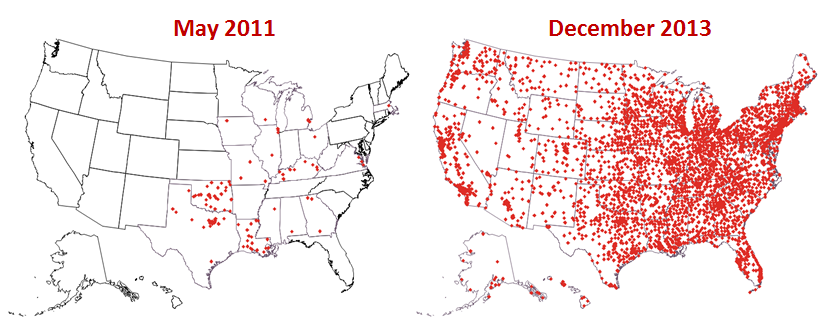
\includegraphics[scale=.6]{Objects/QS-Hospitals-Receiving-Payments-for-MU-and-Adoption.png}
    \caption*{Source: HealthIT.gov}
    \label{fig:meanuse}
\end{figure}

Figure \ref{fig:EPIC} shows a two computer screenshots of what physicians might see in their EHR system. On a daily basis, a physician spends approximately 23.7\%, 17\%, and 15.5\% of their time on documentation, chart review, and inbox management, respectively (\cite{arndt2017tethered}). These are the most time consuming portions of EHR use, according to the same study. In all, if a physician works for 12 hours, they spend roughly 3.2 hours with patients and 5.9 hours interfacing with an EHR. Despite a large amount of time spent with them, physicians still continue to report frustration over EHR use. The most time consuming functions are also reported as the most frustrating (\cite{dymek2021building}). A physician still likely spends almost 2 hours a day managing their inbox: deleting duplicate messages, sifting through messages meant for other members of a care team, and searching relevant information (\cite{dymek2021building}). Another common issue physicians face is the lack of usability of EHR systems, that functions either take minutes to locate or even longer to load. Hospitals often provide training upon adoption, but rapid system upgrades and changes make familiarity with the system difficult. Physicians have been voicing concerns over EHR usability since their beginning, indicating that they are likely responding in their behavior as well.

\begin{figure}[ht]
    \centering
    \caption{Screenshot of EHR System}
    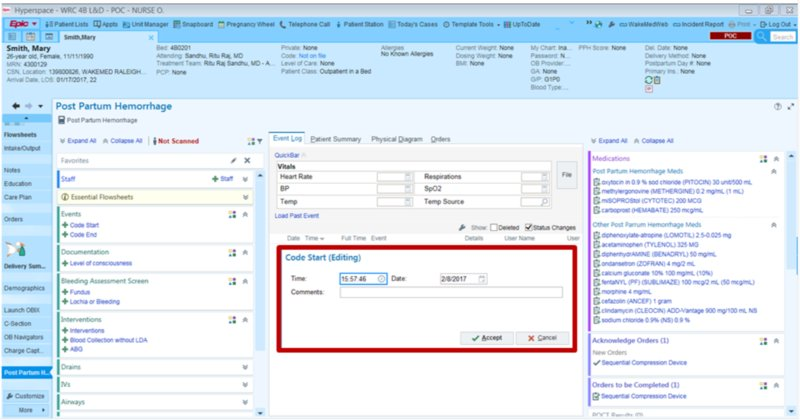
\includegraphics[scale=.4]{Objects/epic-ehr-screenshot.jpg}
    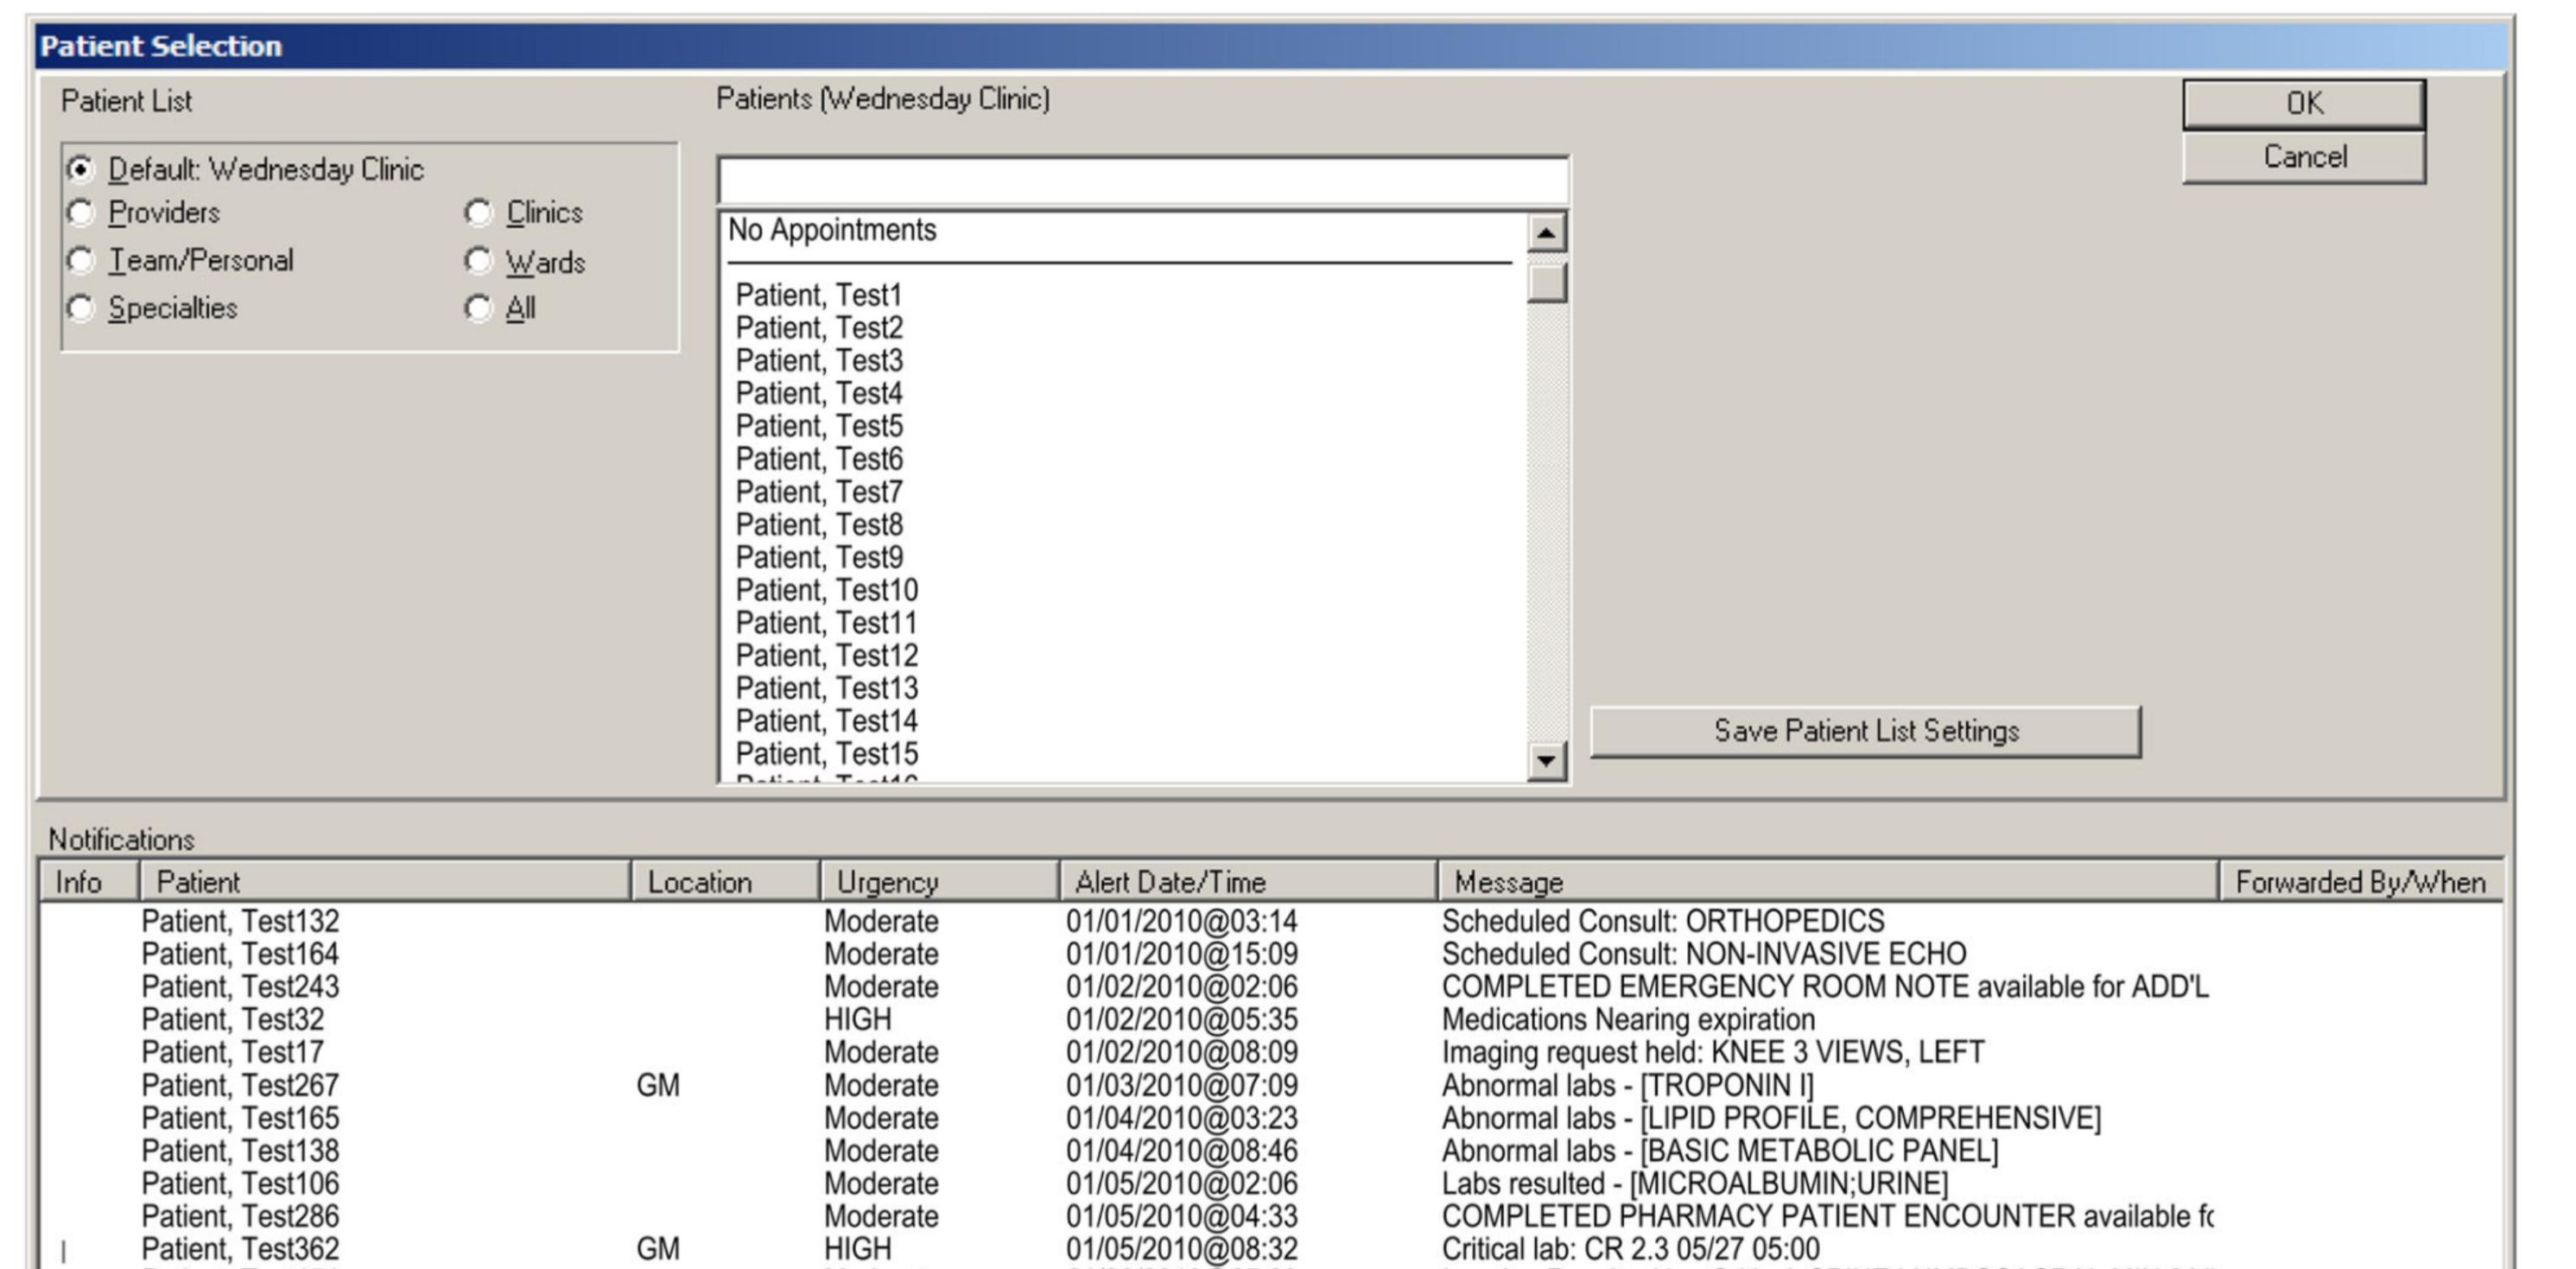
\includegraphics[scale=.115]{Objects/EHRimage2.jpg}
    \label{fig:EPIC}
\end{figure}


\section{Physician Incentives}

This section serves to outline the potential responses of physicians who work primarily in hospitals to EHRs based on the costs and incentives they face. The physician behaviors that I consider in this analysis are closely related and should not be taken as independent. For example, a physician's choice of work setting depends on their previous decision to prolong retirement, and billing activity depends on work setting. Thus, I discuss the behaviors in stages of decision making. 

\subsection{Retirement}

Workers in developed countries tend to plan for formal retirement well in advance. Generally, an exogenous shock to a worker's environment is not expected to change retirement age due to the amount of wealth and planning necessary to formally leave the labor force. Classic retirement models structure the decision of retirement by maximizing expected lifetime utility based on future earnings and retirement benefits, or choosing to prolong retirement only if the expected earnings gain from doing so is positive (\cite{gustman1986disaggregated}, \cite{stock1990pension}). However, physicians typically make this decision differently than workers in other industries. Most physicians plan to retire at age 60, but do not actually retire until age 69 (\cite{collier2017challenges}). When the time to retire comes, many physicians hesitate to abandon patients they have seen over the course of their career. The decision to delay retirement is not financial, but altruistic. Thus, retiring may be in a physician's choice set years before the realized decision to leave the labor force. 

It is important to note that age is the most important factor in the decision to retire, implying that a 35 year old physician has very different incentives than a 65 year old physician, and a technology shock will affect the age groups differently. First, I consider physicians already of retirement age when a new technology is implemented. While payment schemes, wealth, and retirement benefits certainly impact the utility a physician receives from working or retiring, I assume the decision to retire is independent of those things since, on average, those in this age group have already prepared financially to retire. Then, a physician will only retire if the utility from working is less than the utility from retiring, where utility from working depends on job satisfaction and personal life. Exogenous EHR implementation affects the decision to retire through its affect on job satisfaction. If EHRs impose a burden on daily tasks, there is an inverse relationship between EHR exposure and utility from continuing to work. If EHRs make daily tasks easier, there is a positive relationship. Thus, for a physician indifferent between retiring and continuing to work, EHRs induce retirement if they impose a cost in terms of job satisfaction, or induce continued working life if they impose a benefit to job satisfaction. Media articles focusing on interviews with particular physicians suggest that the implementation of EHRs did in fact lead to retirement in older physicians (\cite{ringel_2019}, \cite{loria_2020}), suggesting a negative impact. 

Formal retirement (leaving the labor force altogether) is not the only way for physicians to transition out of a clinical role. There are opportunities for physicians of any age to switch careers towards more administrative roles such as teaching, consulting, or hospital management. While it is unlikely that physicians under 55 are formally retiring, physicians of any age could be career switching. This decision is impacted similarly to the above discussion regarding formal retirement, where a physician who is indifferent between clinical work and career switching can be affected one way or the other based on how EHRs impact job satisfaction of current clinical work. As I discuss in the Data Section, I only observe whether a physician stops seeing Medicare patients, not whether they retire or career switch. Thus, the term "retirement" for the purpose of this paper indicates no longer seeing patients, and makes no assertion about what the physician does afterwards. A physician is said to retire in a given year only if it is the first year in which the physician has no future Medicare claims.



\subsection{Work Setting}

For most physicians, EHRs will not impose a costly enough burden to induce retirement. However, there are other ways physicians might change their behavior under sufficient incentive to avoid the technology. For those who remain practicing in a clinical environment, changing the physical place of work may allow the physician more control over the technologies used in the work environment, affecting overall job satisfaction. Generally, physicians may have the ability to move hospitals, move from a hospital to an office, or work in multiple facilities and shift the composition of patients towards other facilities. I only consider physicians who are classified as a primary care physician and are closely tied to at least one hospital, often referred to as hospitalists or internists (for a detailed discussion of included physicians, see Appendix \ref{app:data}). Some hospitalists work under contract full time for one medical practice, where they have a consistent shift schedule, while others contract themselves out to multiple hospitals, offices, or both. 

First, I consider those who are in a relatively binding contract. For hospitalists under full time contract with a medical practice, the physician is more tethered to the hospital. This could impact the response to EHR implementation in that hospital in two ways: (1) through potentially increased use of the EHR in its initial phases, and (2) limited access to other work settings. A typical contract requires 90 to 120 days termination notice and some contracts include do not compete clauses (\cite{yasgur_by_-_yasgur_2016}), making a shift in work setting costly or excluding it from the choice set. Since these hospitalists are established in their hospital, they work a significant amount of time there. When an EHR is implemented, they may become familiar with it more quickly and be less likely to desire to switch work settings. Alternatively, there are hospitalists that work in multiple hospitals or work in both hospitals and offices. If one hospital implements a costly (or beneficial) EHR, these workers can more easily shift all or some of their work towards (or away from) different facilities to allocate to the place where they gain the most job satisfaction.  


\subsection{Productivity}

There are likely still physicians who are not induced to change their behavior on the basis of retirement or work setting due to EHR implementation. A lack of response could be due to 3 factors: EHRs make no impact on the work environment, EHRs are costly, but not costly enough to shift, or EHRs improve job satisfaction in the current work environment. For physicians who make no physical changes to work environment after EHR exposure, it is natural to assess whether EHRs affect output in current work environment. An important, and heavily debated, aspect of the implementation of EHRs is whether or not they allow users to be more productive. A main purpose of the HITECH Act was to improve efficiency of care, specifically to decrease time spent on administrative burden. Such a decrease implies a change in patient care: either a larger number of patients have access to an appointment, or the same amount of patients receive more face-to-face time with physicians during appointments. Alternatively, because the technology is not hugely user friendly, it may not decrease administrative burden after all.




\section{Data}

Using various linked data sets, I construct a physician-level panel spanning from 2009-2017 which measures physicians' exposure to EHRs over time, outcomes related to physician practice location and billable activity, and other relevant physician, hospital, and practice characteristics. I describe the different data sets used to construct the panel below. I include a detailed outline of data and variable construction in Appendix \ref{app:data}.

\subsection{MD-PPAS}

The Medicare Data on Provider Practice and Specialty (MD-PPAS) is a database of physicians which details claim counts, physician specialty, and practice location from 2009-2017. Included in the MD-PPAS is physician NPI, primary and secondary specialties, both patient and total billing counts in up to 12 different zip codes, and fraction of patients in different settings such as office, inpatient or emergency room. I first limit the sample of physicians based on specialty type. My analysis relies on EHR implementation in hospitals. Thus, I only include physicians who reported their primary specialty as hospitalist (physician who self-identifies as hospitalist or has 90\% of patients in inpatient setting), internal medicine, general practice or family practice in at least one year. However, I exclude physicians who list themselves as a specialist in all but one year. Since the focus of the analysis is physicians working in hospitals, I also drop physicians with less than 70\% of patients in a hospital setting in all years and I drop physicians with insufficient claim counts to show indications of behavior.

This data includes information on physicians which I use to construct the dependent variables for my analysis. Generally, these include the decision to retire (leave clinical work), the decision to switch to a different work setting, number of patients seen, and overall billing activity. I describe these outcome variables and their construction in detail below in Section \ref{sec:outcome}.


\subsection{Shared Patients}

CMS Shared Patient data records annual information on the number of patients who bill two entities under Medicare from 2009 to 2015. For example, if a primary care physician refers a patient to a specialist, then those two physicians have that particular shared patient in common. The number of shared patients are collected in 30, 90, or 180 day intervals. I focus on the number of shared patient billing two entities in the same day, within a 30 day interval. I employ this data to detect physician who work closely with hospitals and which of those hospitals have implemented an EHR, denoting each physician's exposure to EHRs. This measure of exposure defines various treatment variables for my analysis. I limit the entities by tax-code to only include shared patients for physician-hospital pairs, where the physicians in these pairs match the physicians from MD-PPAS. I am specifically interested in primary care physicians who have a close working relationship with hospitals, who do rounds within at least one hospital. The types of physicians are already limited to primary care, but there still may be office-based primary care physicians in the shared patient data. Therefore, I limit the sample of pairs based on a threshold of same day patients which depends on the number of years the physician appears in the data. I only include physician-hospital pairs who have non-missing data with at least 30 shared patients per year, which gives a threshold of work relationship without excluding physicians who have no claims for a number of years.

\subsection{AHA Survey Data}

Using hospital NPI, I link the physician-hospital pairs from the shared patient data to the American Hospital Association (AHA) survey, which contains information on hospital-level EHR use and other characteristics. I record the first year a physician is exposed to an EHR based on implementation in the hospitals they share patients with. I then aggregate this data to the physician level. Since the Shared Patient data does not extend to 2017 as the MD-PPAS data does, in the analysis I drop physicians who are not treated by 2015 as I do not observe whether they become treated in 2016 or 2017. That is, the data contains no units which are "never-treated".

\subsection{Physician Compare}

Finally, I include a physician's graduation year from Physician Compare. I limit to physicians who graduated before 2005, as anyone who graduated medical school after that will be finishing residency during the span of the data and will exhibit labor market changing behavior which could be correlated to EHR exposure purely because of switching work settings during a time of rapid EHR implementation.

\subsection{Outcome Variables}\label{sec:outcome}

The first dependent variable I consider is the decision for a physician to stop seeing Medicare patients, which I loosely call retirement. This variable is constructed as follows: 
$$\text{retire}_{it}=\mathbbm{1}\{FC_{it}=0 \text{ and retire}_{i,t-1}=0\}, $$
where $FC_{it}=\sum\limits_{j=t+1}^T\text{(claim count)}_{ij}$ is all future claims for physician $i$ in year $t$. Retire is therefore an indicator variable set to one in the first year that a physician has no claim counts at any point in the future \footnote{Alternatively, I could also define retirement using future number of patients. I use claim count for a more conservative measure of retirement, but using patient count yields identical results. In Appendix \ref{app:years}, I limit the sample years to 2009-2015 to ensure sufficient future year of zero claims.}.

Next, I consider whether physicians exhibit behavior that suggests they have shifted setting or location of work. I measure this in the data in three ways. First, I consider the fraction of patients a physician sees in an office-based setting, which is directly available in the data. Second, I construct an indicator variable equal to one if a physician sees a positive fraction of patients in an office-based setting. This binary measure of practice setting offers less variation but captures a more discrete changes in which physicians enter or leave the office-based setting entirely. Third, based on the physician's practice zip code, I form an indicator variable equal to one if the physician's list of zip codes changes from one year to the next. While no single variable directly measures physician movement across hospitals, these three outcomes collectively provide insight into whether physicians desire to shift away from EHRs.

Finally, I consider outcome variables which explore inputs to overall efficiency in health care, the number of patients seen and total billing activity.


\subsection{Summary Statistics}

I show summary statistics for the entire sample in Table \ref{tab:sumstats}. Only 3\% of physicians (approximately 770) retire over the course of the panel. 30\% of the physician-year observations have value one for working in an office in some capacity, with about a tenth of the number of patients being seen in an office setting. By construction, all physicians are exposed to an EHR at some point in the sample, so the variation in treatment variables comes from the timing of exposure. Physicians are typically exposed about one fourth of the way through the sample, but there is a positive number of physicians first exposed in each year from 2009-2015. The average physician is 45 years old, works with 1.5 hospitals and 1.3 systems. 
\import{Table Code}{overall stats.tex}


I also include a table of means comparing physicians younger than 60, at least 60, and physicians who ever retire (who can fall in either age category) in Table \ref{tab:splitstats}. Senior physicians see more patients and work in more hospitals on average than younger physicians. These older physicians also see a larger fraction of patients in an office setting and are more likely to work in an office in general. Finally, physicians in the higher age bracket are less likely to switch zip codes. The age groups are exposed to EHRs in similar ways.


\import{Table Code}{split stats.tex}


In Figure \ref{fig:treatmentgraph}, I present a graph of the variation in treatment over time. In 2009, 32\% of the sample of physicians were already exposed to an EHR. That is, three quarters of the sample had no affiliation with EHRs at the beginning of the sample period. Since I drop any physicians who do not have exposure to an EHR by 2015, 100\% of the sample is exposed by then. The black line represents the average fraction of a physician's hospitals which are utilizing EHRs over time. This shows that, along with becoming first exposed over the sample period, physicians are also seeing EHRs implemented in more of their own hospitals over time.

\begin{figure}[t]
\centering
    \caption{Treatment Variables Over Time}
    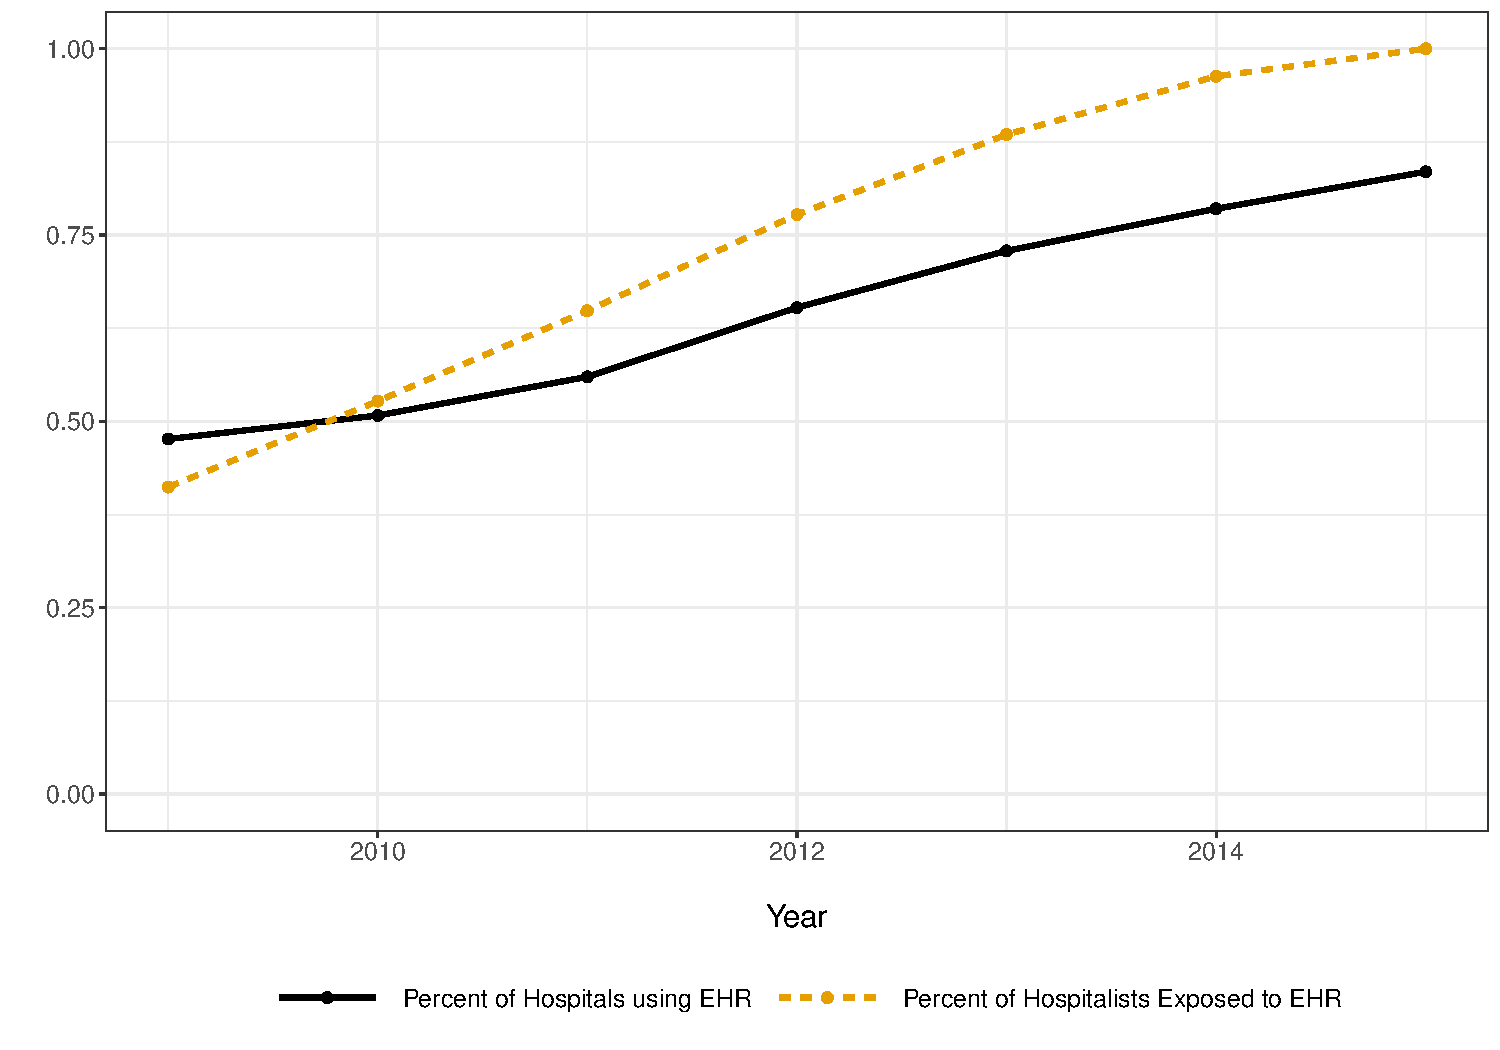
\includegraphics[scale=.45]{Objects/sum_stats_year.pdf}
    \label{fig:treatmentgraph}
\end{figure}



\section{Empirical Strategy}

I treat EHR implementation as an exogenous treatment variable, and I seek to estimate average treatment effects of EHR exposure on various physician outcomes. In this setting, treatment effects are heterogeneous across physicians who are exposed in different years since the underlying characteristics of hospitals who adopt in different years may be correlated with the decision to adopt. Therefore, to avoid negative weighting issues this causes in a classical two way fixed effects event study specification, I instead estimate average treatment effects for a specific group $g$ at time $t$: 
$$ATT(g,t)=\mathbbm{E}[Y_t(g)-Y_t(0)|G_g=1],$$
where $G_g=1$ for those in group $g$. A group indicates all physicians treated, or first exposed to an EHR, in the same year. To estimate the heterogeneous treatment effects, I employ the doubly robust estimator established in \citeauthor{callaway2021difference} (\citeyear{callaway2021difference}). Other estimators that similarly address the concerns yield similar results, presented in Appendix \ref{app:estimators}. I also present classical two way fixed effects results with physician and year fixed effects in Appendix \ref{app:estimators}. These results yield similar patterns with slightly smaller magnitudes. 

Once I estimate the $ATT(g,t)$ for each group and year, I aggregate the estimates over groups to a more familiar event study plot. When the dis-aggregated estimates are of value, I present those as well. Further, a weighted average of estimates is taken to provide a single $ATT$ value for each outcome; these values are presented in the notes of each table. Simultaneous confidence bands, calculated using bootstrapped standard errors, are presented. 

\subsection{Assumptions}

There are several assumptions necessary to identify the parameters of interest, $ATT(g,t)$. First, I assume that treatment is not reversed once it occurs. That is, once a physician is exposed to an EHR, they cannot be un-exposed. At the hospital level, this assumption is supported by both the institutional details of hospital EHR implementation and the definition of exposure. An EHR is a costly technology and requires a significant amount of collaboration to implement. A hospital does not have incentive to un-implement an EHR once it is implemented. They may add features or switch vendors, but do not reverse EHR use. This institutional detail is supported by Figure \ref{fig:hosp_treat}, which shows EHR status of a 2\% random sample of hospitals over time\footnote{Note that out of the 81 hospitals included in the random sample, 4 of them show a reversal of treatment status. Upon further inspection, each of these hospitals show such a reversal due to a discrepancy in the coding of whether the hospital uses an EHR partially or fully. Those who use the EHR partially are coded as not fully implementing an EHR since it is not clear whether physicians in the sample would be exposed yet or not. Hospitals with this discretion arre coded as implementing an EHR in the first year that they answered "fully" to the survey question.}. Further, since we think of treatment at the physician level as exposure to the technology, this assumption is satisfied when thought of as whether the physician has ever used an EHR. Once they are exposed to the EHR for the first time, that experience cannot be forgotten. However, when considering the outcomes of patient count and billing activity, it could be that a physician moves from a hospital that uses an EHR to a hospital that does not, affecting the number of claims observed in the data. I investigate this possibility and limit the data to address it in Section \ref{sec:patientcount}. 

\begin{figure}[ht]
    \centering
    \caption{Hospital EHR Adoption Over Time}
    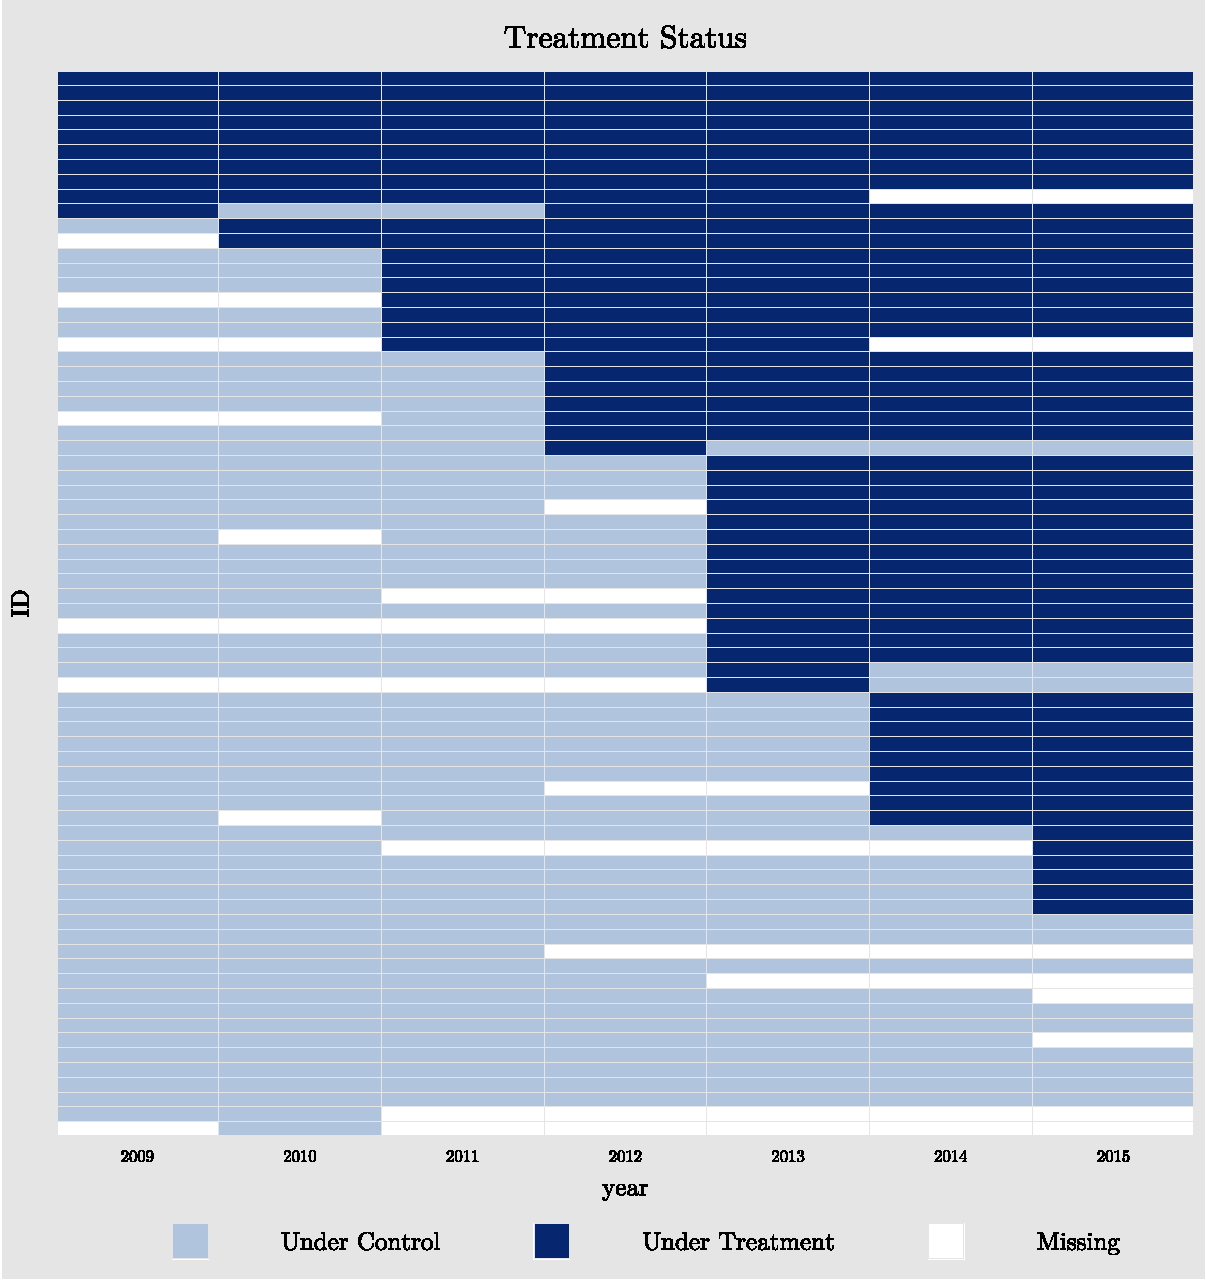
\includegraphics[scale=.7]{Objects/hosp_treat.pdf}
    \label{fig:hosp_treat}
\end{figure}

Second, I assume physicians do not anticipate EHR exposure prior to occurrence. Since the technology has different vendors and varies in capabilities, anticipation may be a concern if physicians learn that the system will be implemented and then do not actually use it until a future period. Generally, even a complex EHR system can be completely set up within a year, and most systems take 6 to 9 months (\cite{uzialko_2021}). Therefore, I proceed in the main specification assuming no anticipation. However, I explore and present results for a one year anticipation period in Appendix \ref{app:anticipation}. 

As is usual in a difference-in-differences framework, I assume a version of parallel trends based on not-yet-treated units. I assume that, conditional on covariates, average outcomes for those treated in group $g$ would have followed a parallel trend as those in groups treated in later periods. This assumption would be violated under external conditions in certain years that may be correlated with labor markets, such as a major recession. The time period I study, 2009-2017, is reassuringly stable. In my analysis, I present p-values for a Wald test of pre-trends. In most cases, there is no evidence of a pre-trend. In cases where a pre-trend could be driving the results, I make no strong claims about the effect of EHR exposure. 

An institutional assumption that I make is that physicians working in EHR-adopted hospitals are constrained to use the technology. My outcomes have two key determinants: the choice of physicians to learn and utilize the technology, and the realized effect of electronic health records themselves. The point of this paper is to identify the second determinant, and thus I assume that when a physician continues to work in an electronic record utilizing-hospital, they utilize the electronic health record system fully. That is, there are no physicians who stay actively working in a hospital but choose not to partake in the electronic health record used by the hospital. It is reasonable to believe that physicians are fully utilizing the EHRs in the hospital they work in, since by 2015 electronic health records were widely implemented and considered unavoidable. An objection to this assumption may be that physicians stay in a hospital, but the hospital hires an employee to do technology work for the physician. In this case, the effects seen could be from having the data assistant instead of EHR use. Thus, I investigate hteir existence further.

\subsection{Hiring Data Assistants}\label{sec:dataass}

One concern with the presented analysis is that any effect could be caused by an outside factor also correlated with EHR adoption in hospitals, such as the existence or hiring of employees with the purpose of utilizing electronic health records on a physician's behalf, which is a way for physicians to continue working in a hospital with an EHR but not experience exposure to the technology. Employees of this type are traditionally referred to as scribes, and are assigned a medical tax ID when working in hospitals. they have the following official titles in tax data: Coding Specialist (Hospital Based), Health Information Technologist and Registered Record Administrator. I will refer to any employee in these categories as a data assistant. In this Section, I investigate whether data assistants were hired in accordance with EHR implementation and whether the presence of data assistants affects physician response to EHRs.  

First, using NPPES data on all NPIs and their tax information, I analyze the existence of data assistants in hospitals. Figure \ref{fig:dataassistant_histogram} presents a frequency plot of the year of activation for every tax code that falls in the categories listed above. The total number of these registered employees is 875, and the first data assistants ever registered were in 2005. From 2005 to 2013, 15-60 more employees were registered each year. The graph is clearly skewed towards later years, where a significant increase in the number of new data assistants occurred in 2014. If hiring data assistants was directly correlated with both EHR implementation and physician frustration, one would expect the increase to occur from 2011-2012, when a majority of physicians first became exposed to EHRs. The results of my main specification are not sensitive to leaving out later years, which is a good indication that the results are not driven by the enumeration of data assistants. 

\begin{figure}[ht]
\centering
\captionsetup{width=.5\linewidth}
\caption{Frequency of Data Assistant Enumeration by Year}
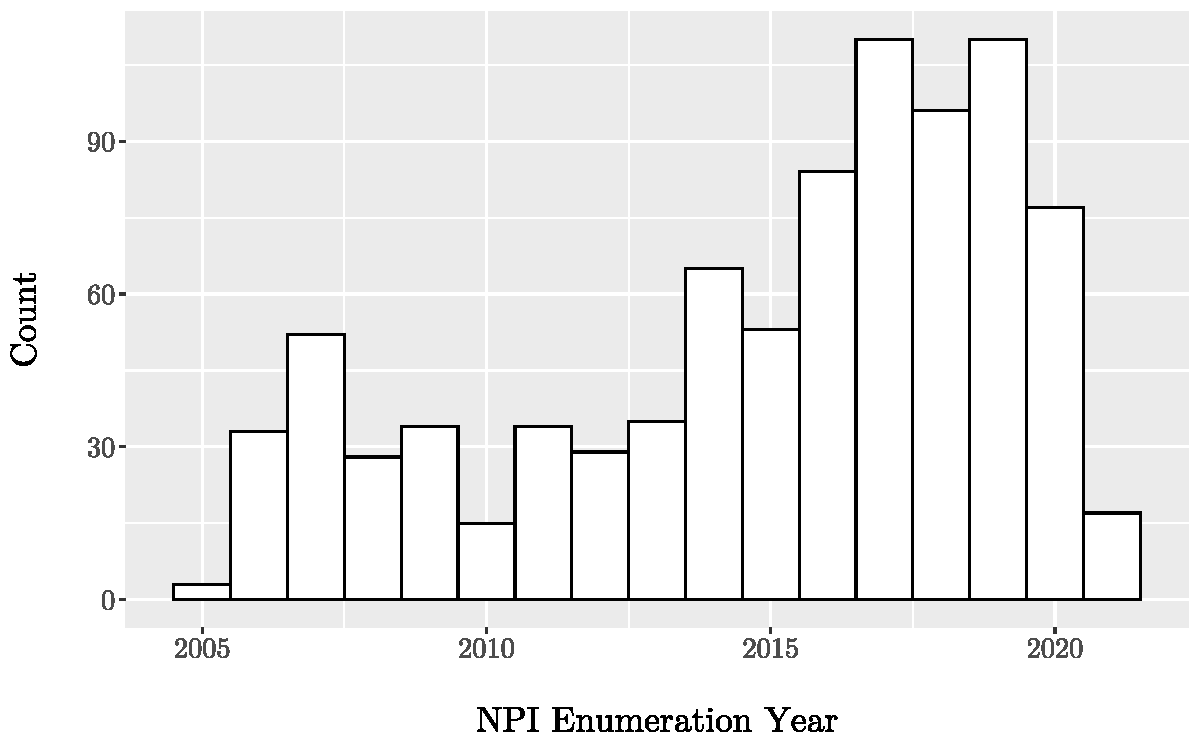
\includegraphics[scale=.5]{Objects/dataassistant_histogram.pdf}
\label{fig:dataassistant_histogram}
\vspace{2mm}
    \caption*{\footnotesize{\textit{Notes:} Histtogram uses NPPES data on the enumeration of certain types of NPIs to estimate the number of new data assistants being hired in each year of my sample.}}
\end{figure}

Further, I investigate the occurrence of hospitals and data assistants sharing patients in the CMS Shared Patient data. I create a list of hospital-years for which the hospital has a positive number of shared patients with a data assistant. I merge this to the physician-hospital pairs and create a physician level variable for whether any hospital worked with is associated with a data assistant. I find that .1\% of physician-year observations are associated with data assistants. This sample of physicians is too small to analyze whether data assistants are more likely with EHR exposure, yielding largely noisy estimates. However, I limit the sample to only physicians not associated with data assistants and find that the magnitude of estimates are similar, albeit more noisy. Details of this analysis are given in Appendix \ref{app:DA}. 





\section{Effect of EHR Exposure on Labor Market Outcomes}

\subsection{Retirement}


In Figure \ref{fig:retirefirst}, I present aggregated group time treatment effects of being exposed to an EHR in any hospital on the likelihood of retirement for the full sample of physicians, as well as split samples for those at least 60 and less than 60 years of age. The top panel suggests that for any age physician, being exposed to an EHR leads to a .002 ppt increase in the likelihood of retiring in both the first and second year after implementation. While this result is numerically small, it is statistically and economically meaningful relative to the proportion of physicians who actually retire in the sample, .02. Thus, relative to the mean, this effect represents a 10\% increase in the likelihood of retirement due to EHR exposure. Considering the magnitude of the decision to retire, it would be alarming to see a numerically large effect on this outcome. A 10\% increase in the likelihood of such a decision is a meaningful jump. While the presented estimates are noisy, the rarity of retirement in the sample combined with the observed precision in the estimates indicates that a positive effect on the likelihood of retirement did occur as a result of EHR implementation.

\begin{figure}[ht]
    \centering
    \caption{Effect of EHR Exposure on Retirement}
    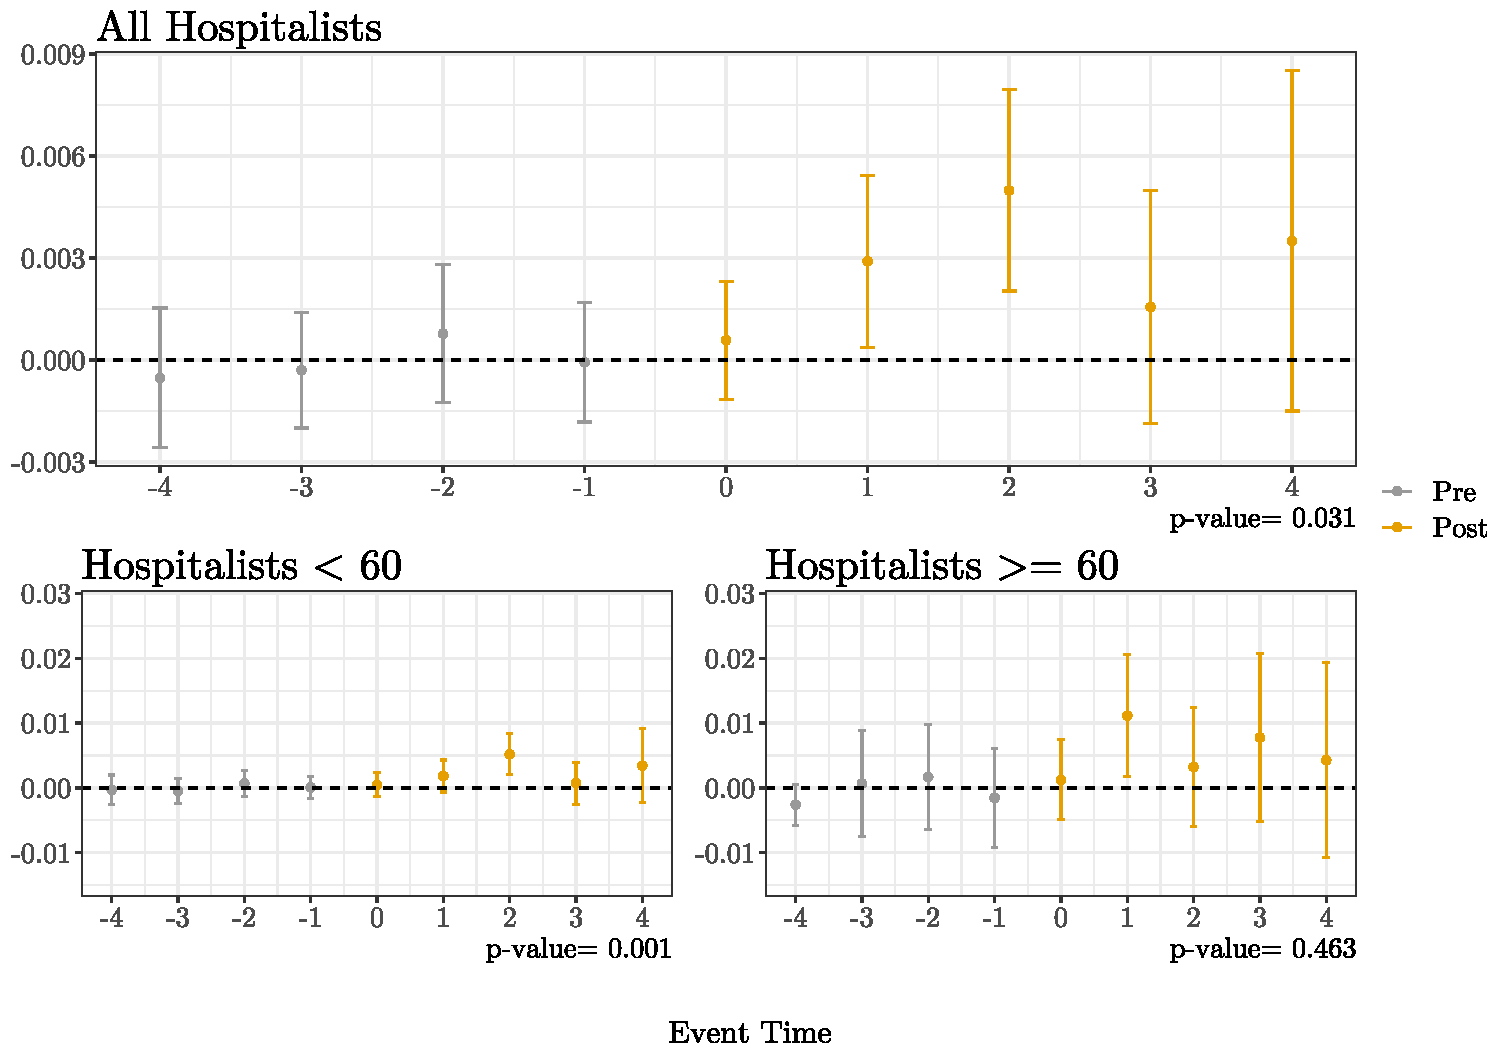
\includegraphics[scale=.65]{Objects/retire_plot.pdf}
    \label{fig:retirefirst}
    \vspace{2mm}
    \caption*{\footnotesize{\textit{Notes:} The top panel shows average group time treatment effects aggregated over groups to an event study plot. The bottom show these results for different subgroups of physicians by age. The p-value listed for each graph corresponds to a Wald test for pre-trends. Confidence intervals shown are simultaneous confidence bands accounting for multiple hypothesis testing. Overall ATT for all, $<$ 60, $>=$ 60 with SE in parentheses: 0.003 (0.0008), 0.002 (0.0009), 0.005 (0.002), respectively.}}
\end{figure}


Next, I examine how the results differ when considering physicians in different age brackets: pre-retirement and typical retirement age. These results are shown in the bottom panels of Figure \ref{fig:retirefirst}, and suggest that senior physicians are driving the positive estimate found above. A physician who is at least 60 years old is .005 ppts more likely to retire after being exposed to an EHR, a 25\% increase relative to the mean. In comparison, physicians less than 60 are far less likely, if at all, to respond to EHR exposure in the first year after EHR exposure. Physicians in the young category have a larger effect on the likelihood of retiring in the second year after exposure relative to the first year. While I do not have data to test this, if young physicians are more likely to switch careers after EHR exposure then it may take one additional year to prepare for that decision relative to retirement.   



\subsection{Work Setting}

 I consider the decision to switch work settings using multiple outcomes. First, I directly investigate the extent to which physicians work in office based setting and whether this changes due to EHR exposure. I use variation in two different variables: (1) an indicator variable equal to 1 if the physician has seen any positive number of patients in an office in a given year, and (2) the fraction of patients a physician sees in an office based setting in a given year. This analysis does not include physicians who retire at any point in the sample, as a zero could indicate dropping out of the data instead of working solely in a hospital. 

I first discuss the effect of EHR exposure on the probability of working in an office setting, shown in Figure \ref{fig:officefirst}. The top panel shows aggregated group time effects for physicians of any age, and suggests that EHR exposure increases the likelihood of working in an office in the year after exposure by .015 percentage points, a 2.6\% increase relative to the mean. This is positive, but somewhat inconsequential effect, both economically and compared to the effect of EHRs on retirement discussed above. Splitting the sample by age reveals that this result is driven by the younger sample of physicians. There is no evidence that older physicians are shifting towards offices. This may be due to senior physicians already being established in some capacity in offices prior to EHR exposure, but is also supported by intuition that older workers are more stuck to their particular work environment.


\begin{figure}[ht]
    \centering
    \caption{Effect of EHR Exposure on Likelihood of Working in Office}
    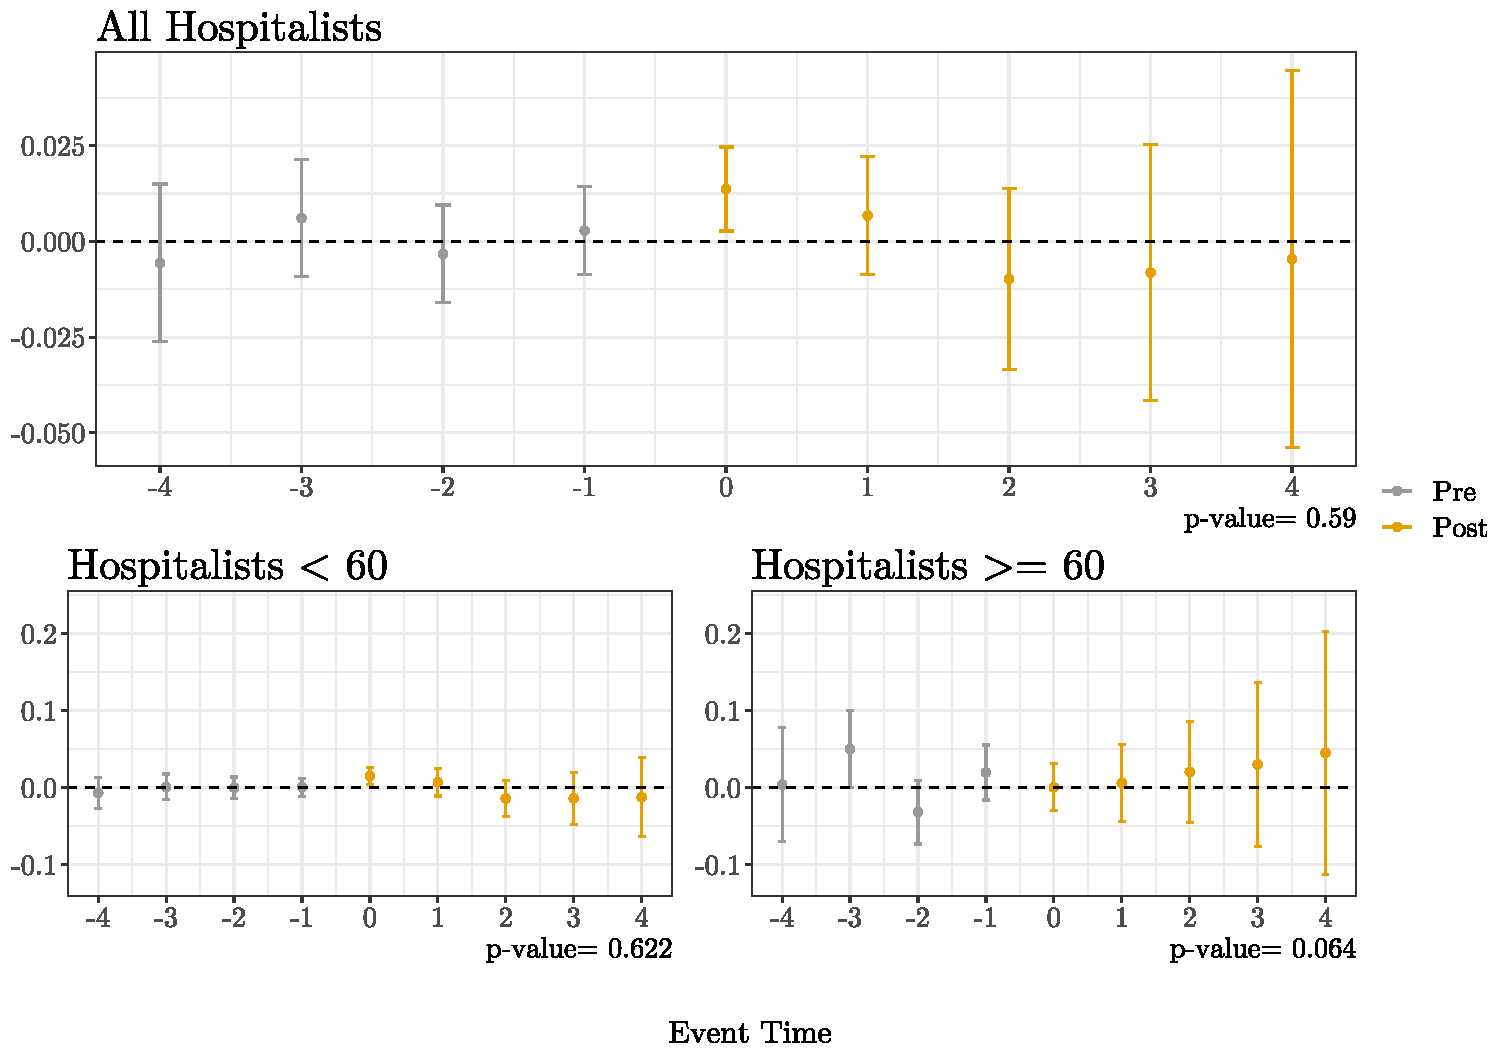
\includegraphics[scale=.65]{Objects/officeind_plot.pdf}
    \label{fig:officefirst}
    \vspace{2mm}
    \caption*{\footnotesize{\textit{Notes:} The top panel shows average group time treatment effects aggregated over groups to an event study plot. The bottom show these results for different subgroups of physicians by age. The p-value listed for each graph corresponds to a Wald test for pre-trends. Confidence intervals shown are simultaneous confidence bands accounting for multiple hypothesis testing. Overall ATT for all, $<$ 60, $>=$ 60 with SE in parentheses: -0.0004 (0.008), -0.004 (0.008), 0.02 (0.02), respectively.}}
\end{figure}

If senior physicians are already established in offices in some capacity, they may be more affected on an intensive margin, the fraction of patients seen in an office relative to hospital or other settings. I show the estimates for this outcome in Figure \ref{fig:officesecond}, where I find no evidence that EHR exposure affects the fraction of patients seen in office settings. This result has varying implications depending on how total number of patients is affected. If total number of patients remains constant, then the absolute number of patients seen in offices is also unchanged. However, if the total number of patients seen (which depends on efficiency in hospitals also) changes, then the absolute number of patients seen in offices necessarily changes in the same direction. I revisit the implications of this result in Section \ref{sec:patientcount}, where I examine the total number of patients as an outcome variable.


\begin{figure}[ht]
    \centering
    \caption{Effect of EHR Exposure on Fraction of Total Patients Seen in Office}
    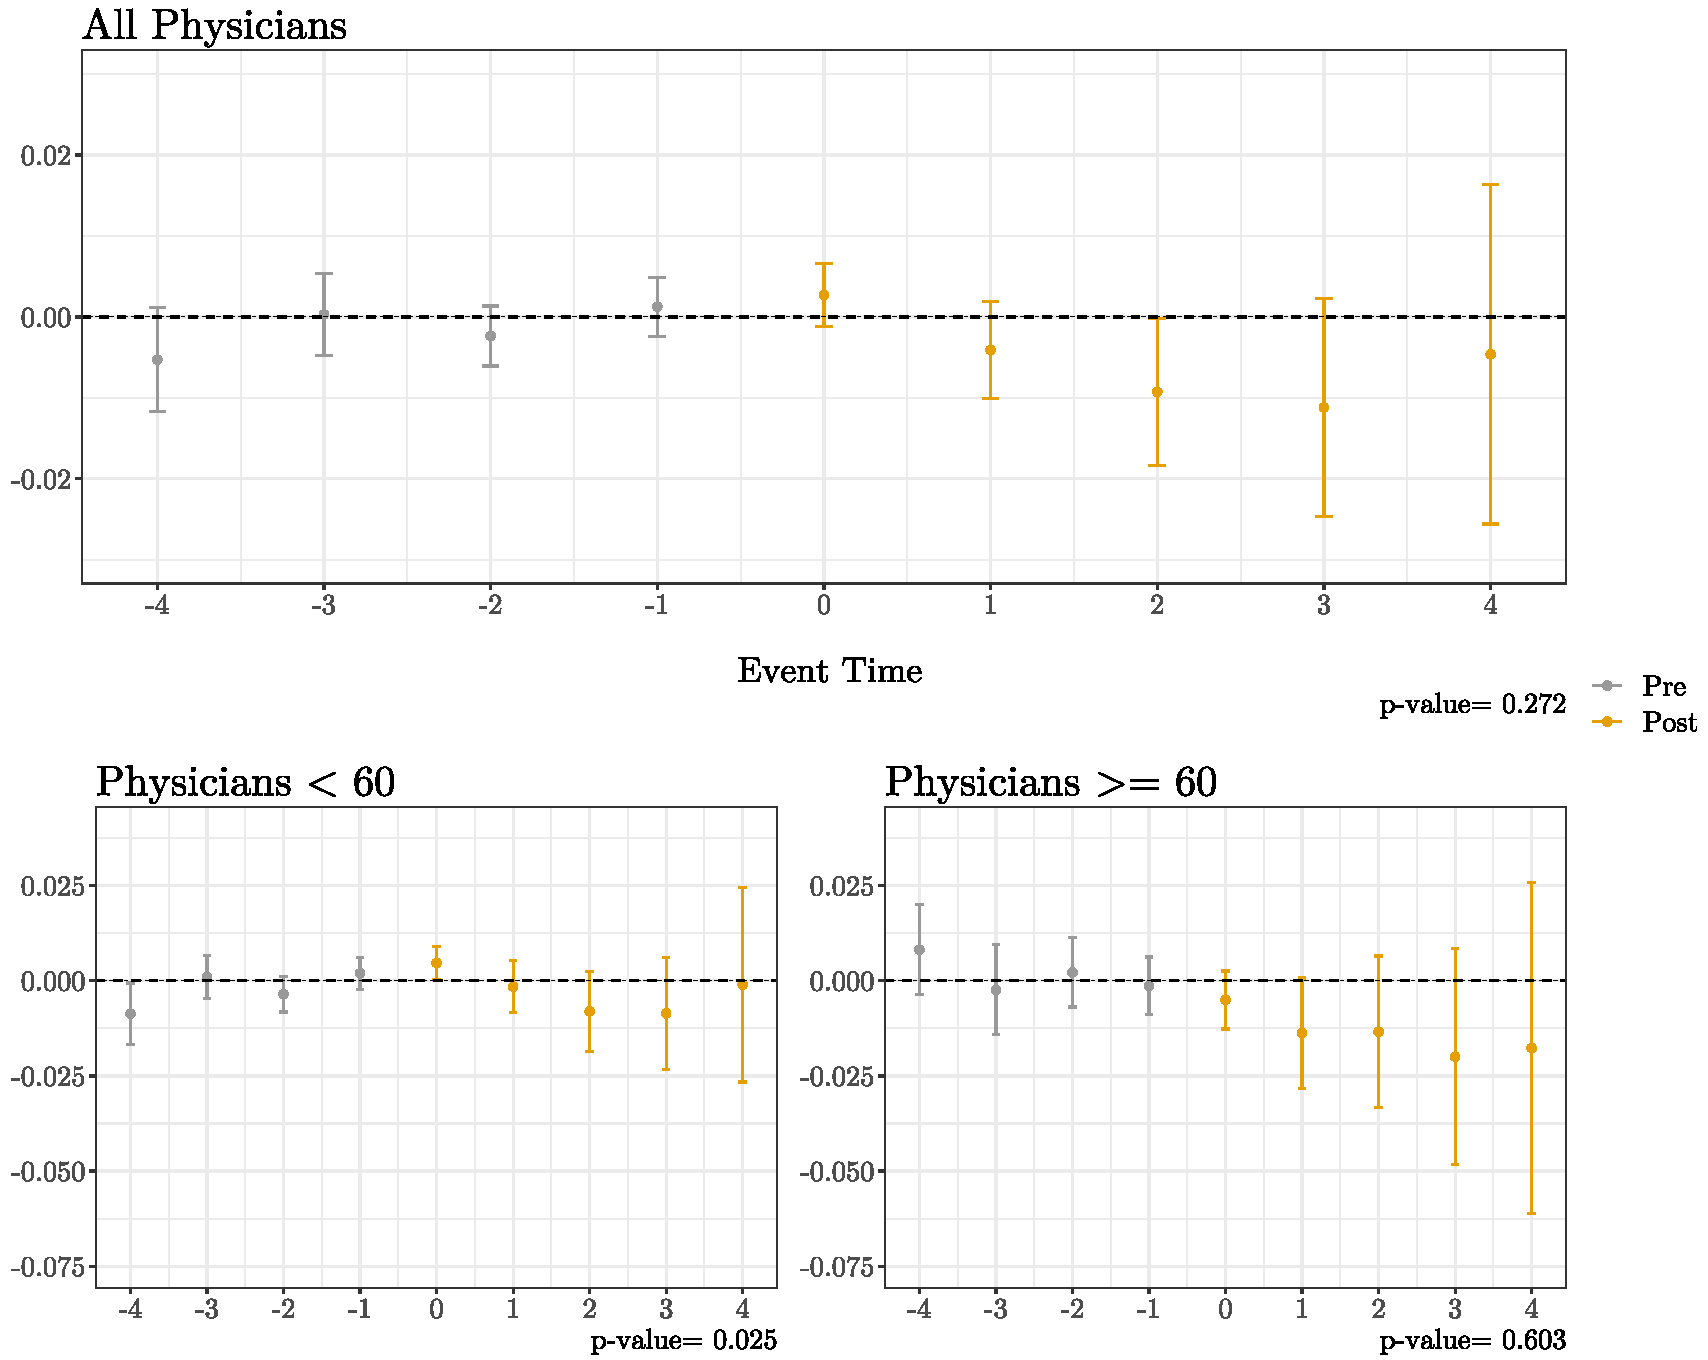
\includegraphics[scale=.65]{Objects/officefrac_plot.pdf}
    \label{fig:officesecond}
    \vspace{2mm}
    \caption*{\footnotesize{\textit{Notes:} The top panel shows average group time treatment effects aggregated over groups to an event study plot. The bottom show these results for different subgroups of physicians by age. The p-value listed for each graph corresponds to a Wald test for pre-trends. Confidence intervals shown are simultaneous confidence bands accounting for multiple hypothesis testing. Overall ATT for all, $<$ 60, $>=$ 60 with SE in parentheses: -0.0003 (0.004), -0.0007 (0.005), -0.006 (0.018), respectively.}}
\end{figure}

The previous results only capture switching behavior which involves office-based settings. A more general way to examine physician switching behavior is to investigate whether the zip codes in which the physicians work is changing, which captures both office and other switching behaviors. Again, I exclude physicians who ever retire. The outcome variable is equal to 1 if the list of primary zip codes (up to twelve of them) changes. This variable is limited in the way it captures switching behavior because multiple scenarios are flagged as changing zip codes: leaving a particular zip code, adding one new zip code but leaving the rest unchanged, or completely changing zip codes. While this is a vague description of behavior, it provides a different insight into changes occurring because of EHR implementation.

The effects of EHR exposure on zip code switching over time are shown in Figure \ref{fig:zip}. While there is a statistically positive effect in the first 2 years of exposure, there is an upward sloping pre-trend that is probably driving this. Thus, I make no claim that EHR exposure is leading physicians to switch zip codes.

\begin{figure}[ht]
    \centering
    \caption{Effect of EHR Exposure on Likelihood of Changing Zip Codes}
    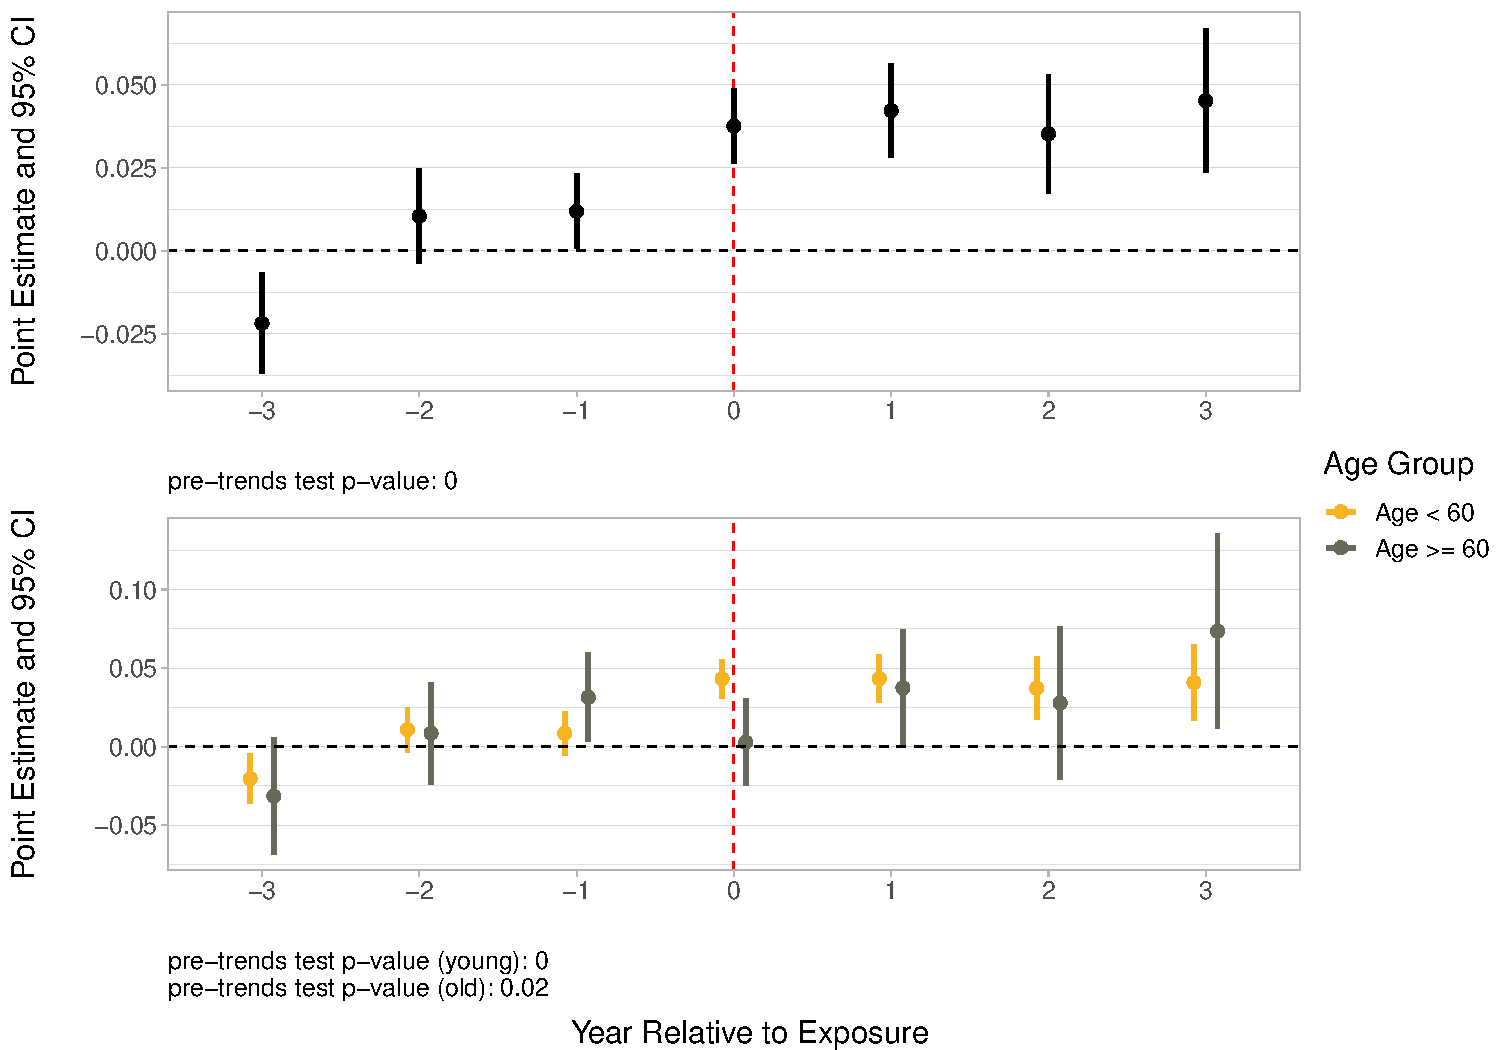
\includegraphics[scale=.65]{Objects/zip_plot.pdf}
    \label{fig:zip}
    \vspace{2mm}
    \caption*{\footnotesize{\textit{Notes:} The top panel shows average group time treatment effects aggregated over groups to an event study plot. The bottom show these results for different subgroups of physicians by age. The p-value listed for each graph corresponds to a Wald test for pre-trends. Confidence intervals shown are simultaneous confidence bands accounting for multiple hypothesis testing. Overall ATT for all, $<$ 60, $>=$ 60 with SE in parentheses: 0.045 (0.006), 0.046 (0.007), 0.042 (0.018), respectively.}}
\end{figure}

A limitation in this analysis is that physicians may shift work behavior due to the organization of the hospital system changing. For example, a hospital may acquire a smaller practice and send physicians to work there for a period of time. If this acquisition is correlated with incentives to adopt an EHR, then the effect I find is biased upward. Since I do not find strong evidence for switching behavior, I leave this question to future research.




\subsection{Patient Count and Billable Activity}\label{sec:patientcount}

For both patient and claim count, if the sample includes physicians who shift place of work, this may lead to biased estimates since a physician could switch hospitals due to an EHR and then change practice behavior due to the move, not due to the EHR. Thus, I limit the sample to only physicians who work with the same one hospital through the entire sample. These physicians do not retire or see patients in another hospital. Thus, when an EHR is implemented, the physician remains utilizing the EHR for the remainder of the period. 

The effect of EHR exposure on patient count is shown in Figure \ref{fig:patient}. For physicians of any age, patient count increases by 11.5 patients in the year of EHR exposure, 24 patients in the year after exposure, 15.3 patients in the second year after exposure, and then no effect after the second year. These results translate to a .5-1\% increase in the number of patients seen relative to the mean. As with other outcomes, this result is totally due to changes by the younger group of physicians. While there is a statistically larger effect for younger physicians relative to senior physicians (who likely take longer to adapt to technology changes), the observed effect is not largely meaningful. 

\begin{figure}[ht]
    \centering
    \caption{Effect of EHR Exposure on Patient Count}
    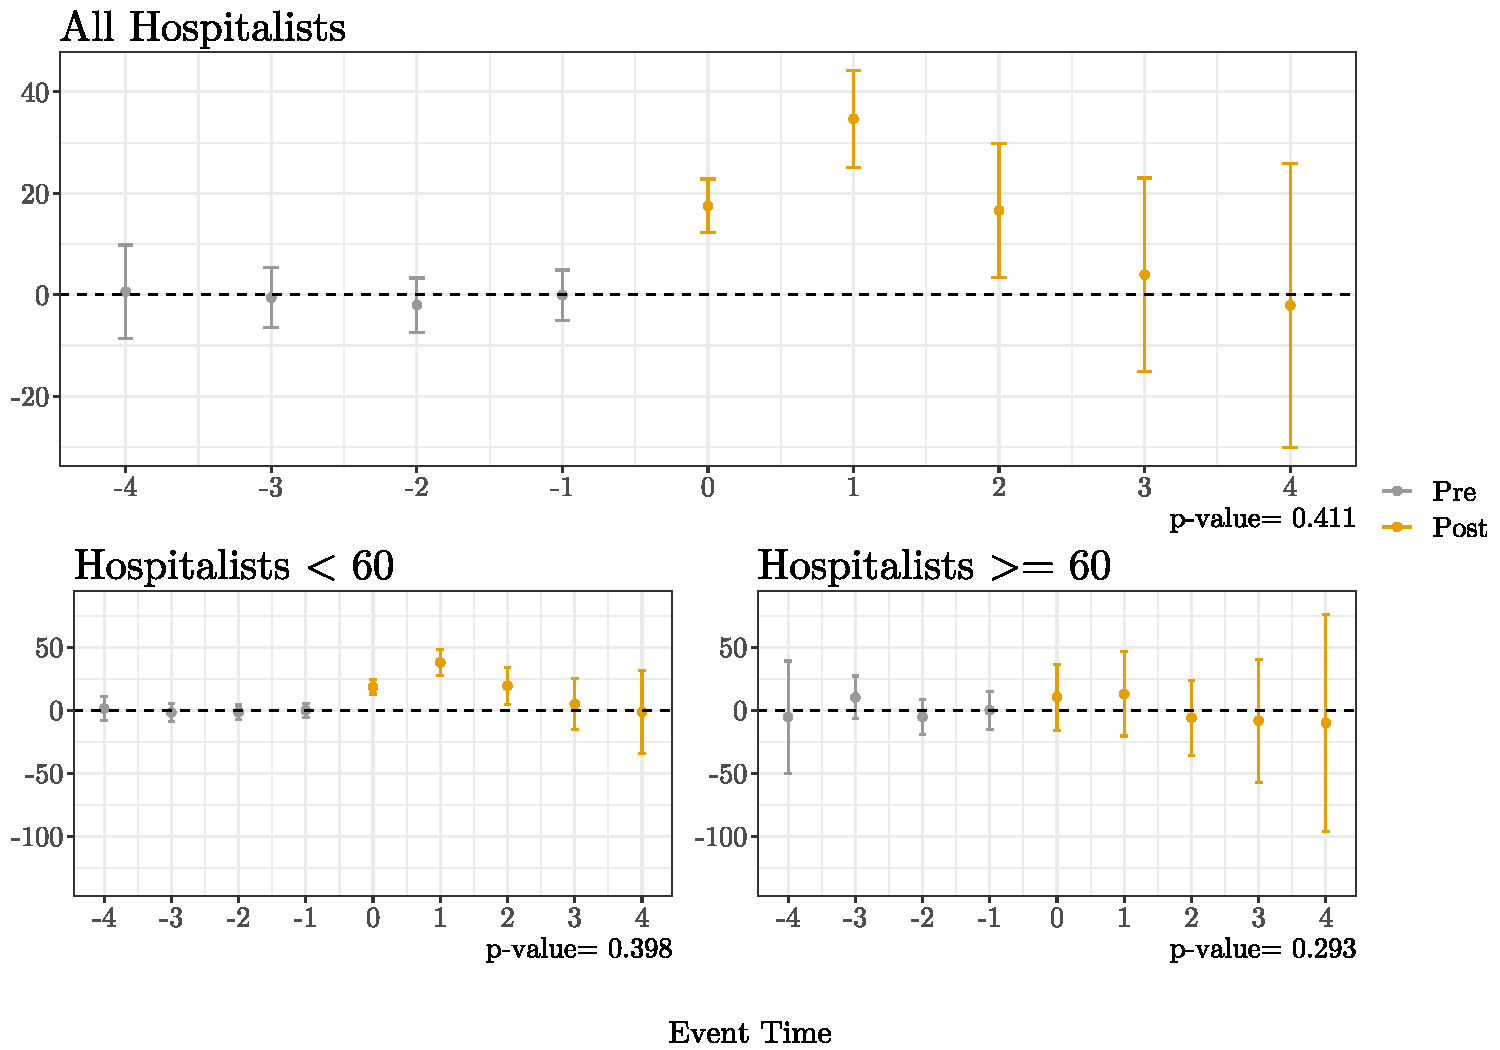
\includegraphics[scale=.65]{Objects/patient_plot.pdf}
    \label{fig:patient}
    \vspace{2mm}
    \caption*{\footnotesize{\textit{Notes:} The top panel shows average group time treatment effects aggregated over groups to an event study plot. The bottom show these results for different subgroups of physicians by age. The p-value listed for each graph corresponds to a Wald test for pre-trends. Confidence intervals shown are simultaneous confidence bands accounting for multiple hypothesis testing. Overall ATT for all, $<$ 60, $>=$ 60 with SE in parentheses: 14.1 (4.6), 15.8 (5.4), -0.29 (13.0), respectively.}}
\end{figure}

Patient count is also driven by demand for health care. A major change in the U.S. health care system, the Affordable Care Act (ACA) was passed in 2010 and took effect in 2014 for the majority of states that partook. If my results are driven primarily by the group of hospitals who implemented EHRs in 2014, one might be concerned that the legislation may be driving the results. The ACA has potentially opposing effects on Medicare patients: Medicare patients may be crowded out by an increased demand in Medicaid patients, or the small changes to Medicare may have led to an increase in utilization from the Medicare population. A recent study found no negative spillovers to the Medicare population due to the ACA (\cite{carey2020impact}), suggesting that demand change is not driving my results. Further, I present average group time treatment effects for each treated group in Figure \ref{fig:patientgroup}. Each group shows the same pattern of a small increase in patient count in the first 0-2 years after implementation. 

\begin{figure}[ht]
    \centering
    \caption{Effect of EHR Exposure on Patient Count by Group}
    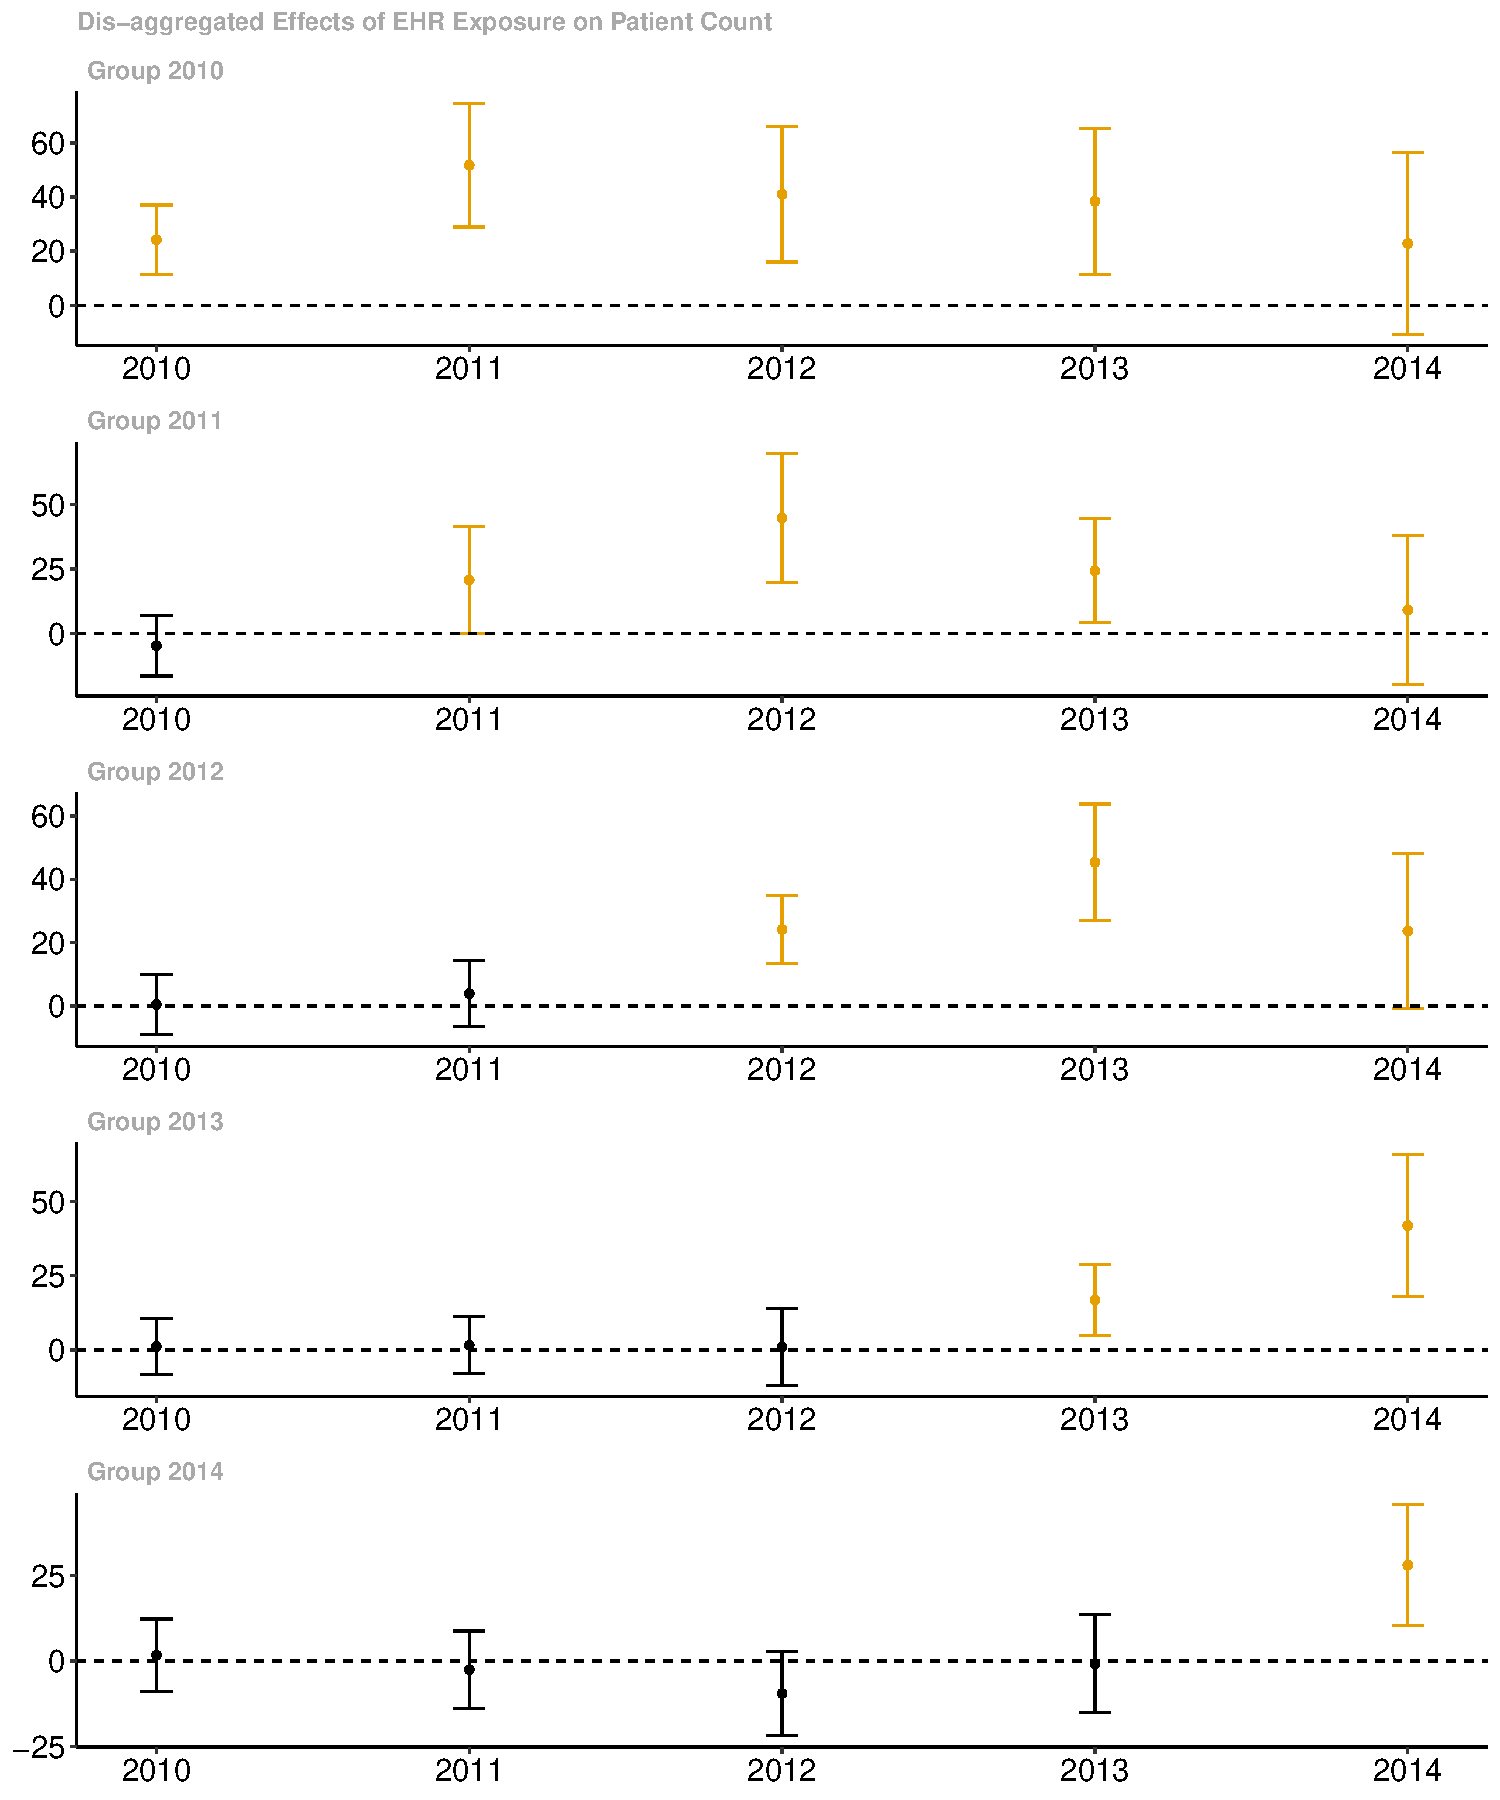
\includegraphics[scale=.47]{Objects/patient_group.pdf}
    \label{fig:patientgroup}
    \vspace{2mm}
    \caption*{\footnotesize{\textit{Notes:} Plot shows average group time treatment effects for each treatment group.}}
\end{figure}

Total patient count is directly related to the fraction of patients seen in an office setting. For younger physicians, since the total number of patients increases in the first couple of years after exposure, the absolute number of patients seen in offices increases as well. That is, it seems that younger physicians are shifting a positive amount of work towards offices but still able to increase productivity in the time spent in the hospital, thus the null effect on fraction of office patients. 

EHRs may affect physician incentives in such a way that billing activity changes differently from patient count. If, for example, EHRs reduce the administrative burden of filing extra claims, then physicians might increase the things they bill for whether the amount of patients has changed or not. On average for the entire sample, claim counts are roughly 5.5 times the number of patients seen in a year. Shown in Figure \ref{fig:claim}, young physicians increase claim count by 37 in the year of exposure and 96 in the year after exposure, 3-4 times the increase in patient count. Thus, billing activity increases proportionally less than average. EHRs do not seem to be facilitating more billable activity. 

\begin{figure}[ht]
    \centering
    \caption{Effect of EHR Exposure on Claim Count}
    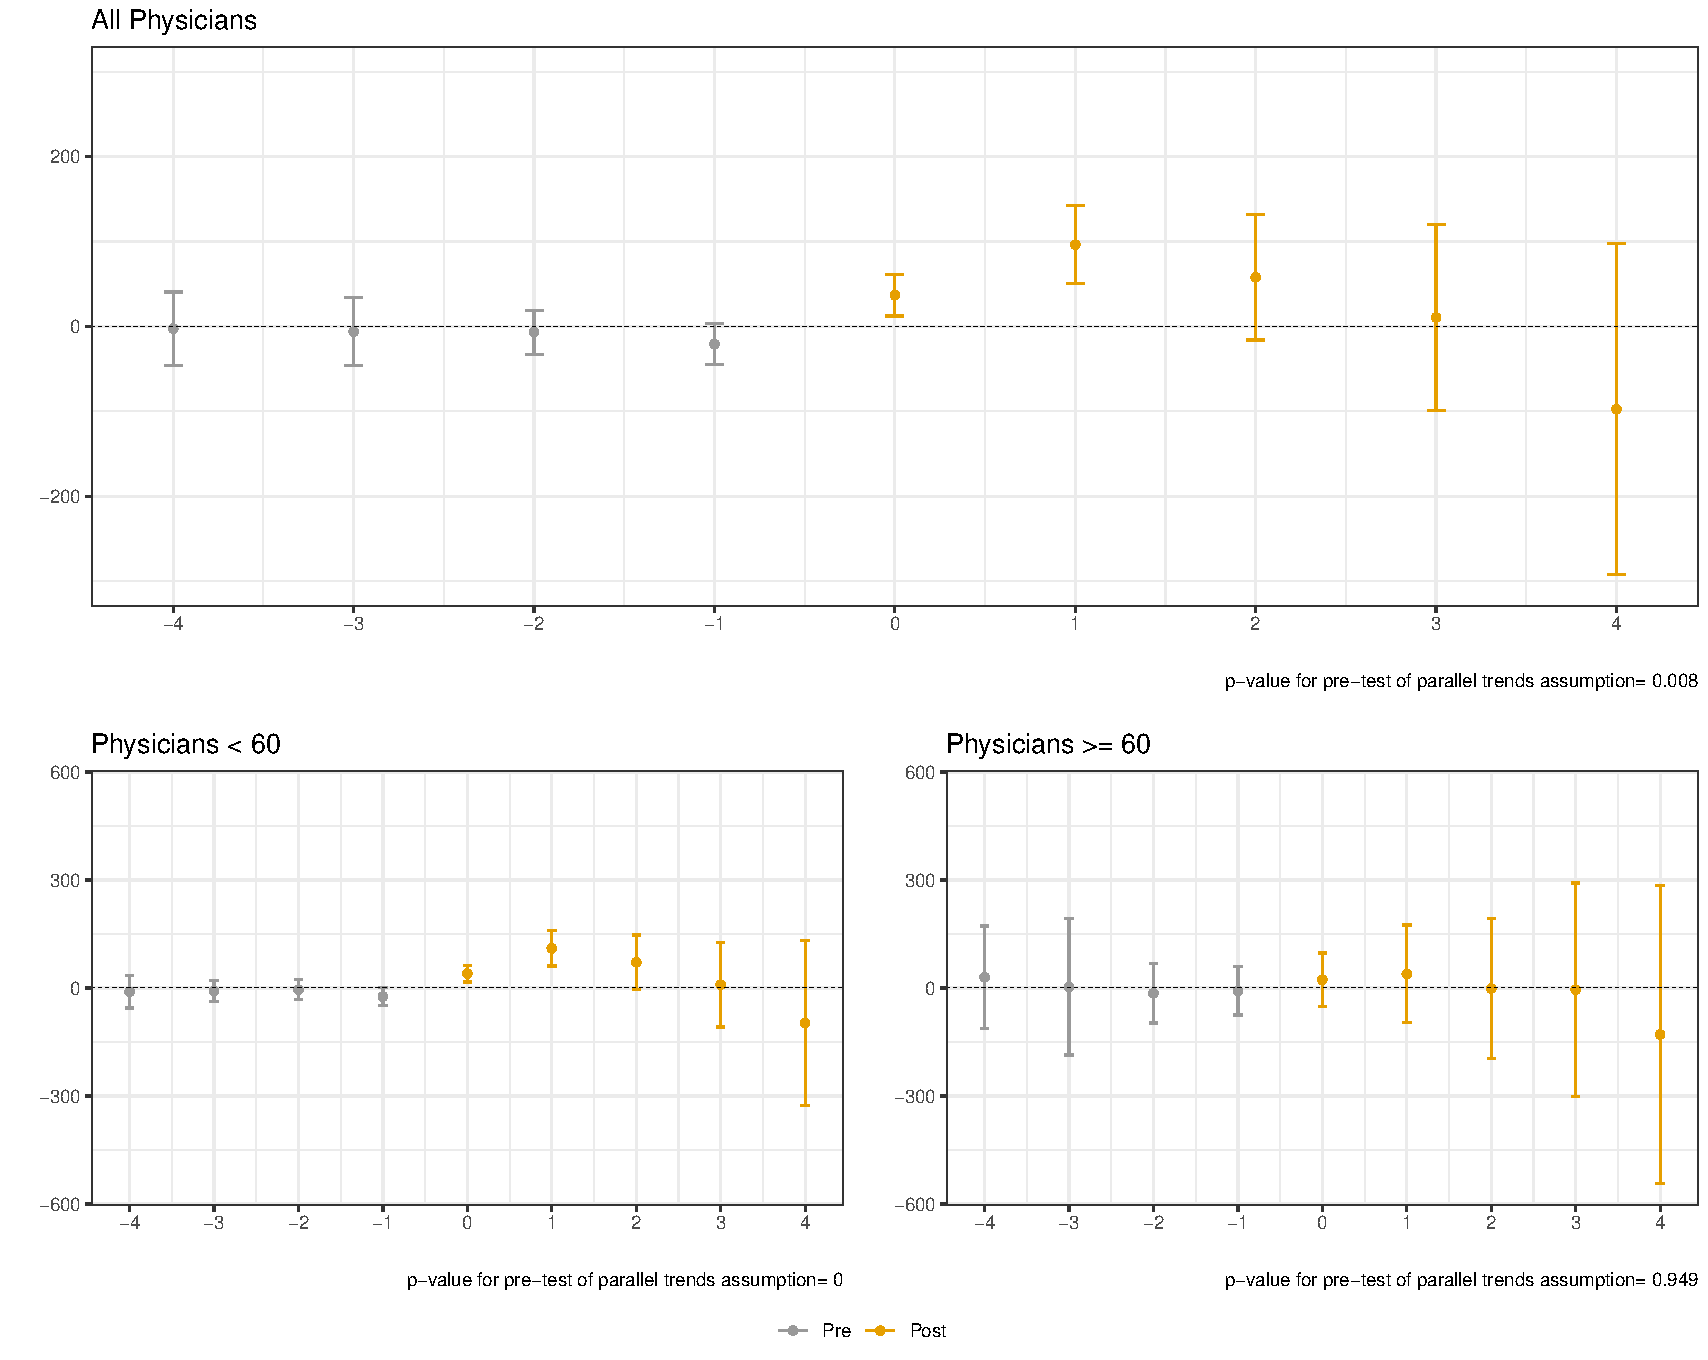
\includegraphics[scale=.65]{Objects/claim_plot.pdf}
    \label{fig:claim}
    \vspace{2mm}
    \caption*{\footnotesize{\textit{Notes:} The top panel shows average group time treatment effects aggregated over groups to an event study plot. The bottom show these results for different subgroups of physicians by age. The p-value listed for each graph corresponds to a Wald test for pre-trends. Confidence intervals shown are simultaneous confidence bands accounting for multiple hypothesis testing. Overall ATT for all, $<$ 60, $>=$ 60 with SE in parentheses: 4.04 (33.89), 25.77 (31.26), -161.06 (133.35), respectively.}}
\end{figure}


\subsection{Late Adopters as Comparison Group}

In the observed results above, if EHR exposure affects physician behavior, the effect occurs in the first 0-2 years after exposure. Almost all specifications point to the effect of EHR exposure to become null in the 3-4 years after exposure. One reason for this may be the composition of the hospitals which adopt at different times. Consider event time $t+4$. The physician included in the estimation for this coefficient are those exposed in 2010 compared with those who did not adopt until 2015, implying that the underlying hospitals implemented EHRs in either 2010 or 2015. It is likely that the group of hospitals who adopted in 2015 are compositionally different than early adopters, especially if poorer hospitals adopted later. For this reason, I have focused discussion of results on the immediate years after exposure when hospitals the comparison groups are more comprehensive. 


\section{Physician Influence of EHR Decision in Hospitals}

Another way physicians may avoid EHR exposure is to exhibit decision making power to either delay or encourage EHR implementation in hospitals. This would make the binary treatment variable endogenous, biasing the results of the main specification, as it includes physicians who are selecting into their own exposure. After the sample period ends, the government began penalizing hospitals for not using health information technology meaningfully, so implementation eventually occurs across the board. However, during the sample, physicians may impact the timing or occurrence of implementation. I address this question by limiting the sample of hospitals in a meaningful way, only including those hospitals which are considered to have low vertical integration with physicians. That is, physicians are employees and less likely to be decision makers. I then redefine exposure as when a physician is exposed to an EHR in low integration settings. I present details of how I define integration and results for this specification in Appendix \ref{sec:endog}. In general, group time estimates are similar to those in the main specification, with the exception of the probability of working in an office setting, which may indicate some correlation between EHR adoption in high integration settings and acquisition of physician offices. 


\section{Conclusion}

In this study, I analyze the effect of implementing a now-common technology in hospitals, electronic health records, on various physician labor market outcomes. This technology has been controversial and debated as a burdensome load on physicians that may contribute to physician burnout, and therefore patient outcomes. The interaction between health information technology and labor markets is vastly important as the technology is continually legislated and growing each year.

I utilize data on shared patients, hospital EHR use, and physician claim activity. Using an event study framework, I find that physicians of all ages who work in hospitals are more likely to stop seeing Medicare patients altogether when exposed to an EHR in a hospital, where those of retirement age have an even larger increase relative to younger physicians. Further, I find limited evidence that physicians are switching work settings, but that this may be driven by hospital incentives instead of physician incentives. Finally, physicians who remain in the labor force increase both number of patients seen and billing activity, but billing activity per patient decreases with EHR exposure. 

The implications of these results are threefold. First, a surge of experienced physicians left the labor force in a concentrated number of years due to EHR exposure, potentially worsening access to care, especially if these physicians are in rural settings. In a field where younger physicians learn a lot by watching those more experienced than them, this particular loss may have long term negative effects on patient outcomes, but this is a question left to future research. Further, physicians are exhibiting behavior that suggests they incur switching costs to avoid burdens externally placed on them. This has implications when considering the current policy movement towards regulated care, that physicians may go to extreme measures to avoid such regulation. Finally, these results speak to the ongoing debate of whether EHRs are generally beneficial to its users. While the technology may be a burden, physicians are able to see more patients because of their use, and are not more incentivized to over-bill. 

This paper contributes to our understanding of health information technology by providing empirical evidence of the theoretically ambiguous physician response to electronic health records being rapidly implemented in hospitals. This contribution is relevant to EHR vendors, hospitals, and policymakers who are involved in further implementation of complex technology. 




\clearpage

\renewcommand*{\bibfont}{\footnotesize}

\printbibliography

\clearpage


\appendix

\section{Data}\label{app:data}

This section details the process of creating the data set used in the analysis of the main paper. 

\subsection{Physician Specialties by Tax Code}\label{sec:taxcode}

I begin by connecting every National Provider Identifier (NPI)\footnote{Data can be downloaded from \hyperlink{https://download.cms.gov/nppes/NPI/Files.html}{\text{https://download.cms.gov/nppes/NPI-Files.html}}} to a description of their tax code\footnote{Data can be downloaded from \hyperlink{https://nucc.org/index.php/code-sets-mainmenu-41/provider-taxonomy-mainmenu-40/pdf-mainmenu-53}{\text{https://nucc.org/index.php/code-sets-mainmenu-41/provider-taxonomy-mainmenu-40/pdf-mainmenu-53}}}. I then categorize NPIs by key words in their tax code description. Any description containing ``Internal Medicine", ``Hospitalist", ``Family Medicine", or ``General Practice" is classified as a primary care physician (PCP), and any description containing ``hospital" is classified as a hospital. I create two data sets, one containing only PCPs and one containing only hospitals. These data are saved to use in identifying the relevant NPIs in the CMS Shared Patient Data. 



\subsection{CMS Shared Patient Data}\label{sec:sharedpat}

For years 2009-2015, the CMS collected detailed information on the number of Medicare patients shared between any two NPIs within 30, 90, or 180 day intervals\footnote{Data can be dowloaded from \hyperlink{https://www.nber.org/research/data/physician-shared-patient-patterns-data}{https://www.nber.org/research/data/physician-shared-patient-patterns-data}}. I use data that captures shared patient activity in 30 day intervals. I merge the shared patient data to the filtered tax code data created in Section \ref{sec:taxcode} to identify NPIs who are either PCPs or hospitals. I filter the pairs to include one physician and one hospital; there are 12.6 million of these pairs. Some pairs are duplicates from the hospital being listed first or second in the shared patient data. I combine duplicates into one observation, summing the same day count variable. Once duplicated are removed, there are 7.1 million observations. Most of the pairs have very few shared patients, which is not indicative of the physician working inside the hospital. I drop any pairs who do not have at least 30 shared patients in the same day per year the pair appears in the data. The final list of pairs consists of 1.3 million observations. 

\subsection{Pair-Level Variables}

I combine the physician-hospital pairs created in Section \ref{sec:sharedpat} with various data sets for hospital or physician level information. First, I merge to CMS Physician Compare\footnote{Data can be downloaded from \hyperlink{https://data.cms.gov/provider-data/dataset/mj5m-pzi6}{https://data.cms.gov/provider-data/dataset/mj5m-pzi6}} for information on each physician's graduation year and gender. This data contains more information on physician quality, but I am limited to time-invariant information since Physician Compare spans 2012-2015 and 2010-2012 is a time of major EHR implementation. I drop any physicians who graduated medical school after 2004, since graduating after that means leaving residency or graduating during the span of my main data, 2009-2017, and potentially exhibiting labor market changes that seem associated with EHRs but are not. 

For hospital level variables, I use an AHA-NPI crosswalk to merge the pairs to the Annual Hospital Administration Survey (AHA Survey) from 2009-2015. The variables I include from this data are a hospital's number of beds, organization type, system ID, and EHR use. There are 4,253 unique AHA hospitals in the shared patient data. I drop any hospitals that aren't in the AHA Survey due to lack of information on EHR use. After limiting the hospitals, there are 780,000 observations of pair-years left. Next, I investigate the hospitals with missing information for EHR use. There are 89 hospitals in the data who never answer the survey question about EHR use; I drop these hospitals. If a hospital does not answer the survey question in one year, but the year before and after have an identical survey answer, I fill in the missing year of information. Then there are 4,253 observations with missing data for the EHR survey question. I make a further limitation to hospitals with at least 10 beds. There are only 58 unique hospitals in the data with less than 10 beds, and these are likely very different from the rest of the sample of hospitals. Then, I create a physician-level variable which captures the average number of beds in the hospitals they work with in each year. I sum a physician's same day count over their hospitals in a given year to create a physician level patient count variable. I also create this variable only for hospitals who are using an EHR and only for hospitals who are not using an EHR.

I merge the remaining pairs to an additional survey, the AHA IT Supplement, only sent to hospitals who reported using an EHR. There are more detailed questions in this survey including the EHR vendor, and the ranking of documentation and decision making features the hospital uses. There is a lot of missing data in this survey, which is why I do not use it in my main analysis. 

I use the general survey question about each hospital's EHR use to define my key treatment variable. The survey asks the extent to which the hospital utilizes an EHR and allows for three answers: not at all, partially utilize an EHR, and fully utilize an EHR. I create a binary variable equal to one if the answer is fully utilize, zero otherwise. The data will be aggregated up to the physician level due to physician level outcome variables, so I first transform the pair-level EHR variable into a treatment variable at the physician level. I create a variable capturing the first year that at least one of a physician's connected hospitals uses an EHR. For the endogeneity discussion in Section \ref{sec:endog}, I create a similar variable but only count a physician as exposed if a hospital categorized as "low-integration" adopts an EHR. The level of vertical integration between hospital and physician is defined as in \citeauthor{dynan1998assessing} (\citeyear{dynan1998assessing}) using the organization type of the hospital. Hospitals classified as IPA or PHO are low-integration, and any other type is high0integration. I also create a variable that captures the fraction of hospitals a physician works with that use an EHR, which varies on the dimension of EHR use and on number of hospitals worked with. Finally, the last variable I create before aggregating to the physician level is an indicator for whether the physician works with the same set of hospitals through the entire sample. I create this variable by comparing a physician's number of hospitals in each year to the maximum number of hospitals they ever work with. If there is any year in which the a physician's number of hospitals is less than the maximum number of hospitals they ever work with, the indicator for never having a new NPI is set to 0. I use this variable to limit the sample in Section \ref{sec:patientcount}. 

Finally, I aggregate to the physician level by only keeping variables that do not vary by hospital. The variables in the physician level data are year, physician NPI, graduation year, average number of beds in hospitals worked with, years of experience, number of hospitals, fraction of hospitals with EHR, minimum year exposed to EHR, minimum year exposed to EHR in low integration hospital, number of systems, patient count, patient count in EHR hospitals, patient count in non-EHR hospitals, and never works with a new NPI. I complete this data to include years 2016 and 2017, but leave time varying variables missing for those years. Thus, this is a balanced panel of physicians. I save this data to be merged with physician labor market activity in Section \ref{sec:appmdppas}.

\subsection{Physician Labor Market Activity}\label{sec:appmdppas}

Using physician NPI, I merge the physician treatment data to Medicare Data on Provider Practice and Specialty (MD-PPAS)\footnote{Information on data located at \hyperlink{https://resdac.org/cms-data/files/md-ppas}{https://resdac.org/cms-data/files/md-ppas}}, which psnas 2009-2017. This data contains variables on physician specialty, Medicare claim counts in various zip codes, unique number of patients seen, fraction of patients seen in specific settings, patient demographics, and physician date of birth. Once the data is merged, I make a further limitation to drop any physicians with less than 20\% of their total patients in a hospital setting. This limitation is to continue ensuring that I am focusing on physicians working in hospitals who will be subject to their EHR use. With this limitation, there are 403,000 observations left in the data. 

Next, I create the dependent variables used in the analysis. The first outcome is whether a physician chooses to retire or not. First, I sum a physicians claim counts across zip codes into one variable for total claim count in a given year. Then, I create a variable that sums up a physicians claims in all future years. In 2009, this variable sums up all claims from 2010-2017, and so on. Then I create a variable for the first year that a physician has a future claim count of zero. However, this counts retirement one year too early. For example, if a physician has no claims from 2014 to 2017, the minimum year variable is set to 2013, but the first year of retirement is 2014. Thus, I add one year to the minimum year variable. I then define the outcome variable, retire, as one if a physician ever retires and the year is equal to the first year of retirement. I utilize a physician level variable for whether they ever retire for sample limitations in analyzing other outcomes. 

The next outcome variables consider level of labor market activity in office settings. The first decision to make is how to handle years where a physician has missing data for claims. A year of missing data can mean the physician had no claims that year, or the observation was removed due to insufficient claims (less than 11). A conservative assumption is to assume a year of missing data means zero claims, thus, I set all missing claim counts to zero. The data already contains a variable for the fraction of patients seen in an office setting, which is used in the analysis, but I further create an indicator variable for whether the physician sees any positive amount of patients in an office setting. 

I also create an indicator variable for whether the physician switches zip codes from one year to the next. The physicians in this data work in up to 12 different zip codes, so I their zip codes into one string variable, a list of all zip codes in a year. I make this variable into wide format: zip list 2009, zip list 2010, ... , zip list 2017.  In year $t$, I define a variable change zip that is equal to one if the zip list in $t-1$ is different from the zip list in $t$, zero otherwise. Finally, the variables for unique patient count and claim count are already defined. This is the final data used in the paper, with 403,020 observations. 



\section{Sensitivity Analysis}

\subsection{Physician Selection into EHRs}\label{sec:endog}

The main specification of the paper defines a binary treatment variable for whether a physician is exposed to an EHR in any hospital they work in. These results are biased if physicians endogenously select EHR exposure, particularly by participating in the hospital's decision to implement. The results do not indicate that this is a huge issue on average, since we would expect physicians not to respond on the margin of retirement or switching work setting if they are choosing to be exposed to EHRs. Especially in larger hospitals, this is unlikely to occur as an individual physician will not have much input to high level decisions. However, as an attempt to provide more evidence of labor market changes as a result of EHR exposure, I provide results for a specification with an alternate binary treatment variable: whether a physician has been exposed to an EHR in a hospital considered to have low vertical integration with physicians. 

I define a hospital's level of integration based on organizational structure, where independent practice associations (IPAs) and physician-hospital organizations (PHOs) are classified as low vertical integration and other organization types are classified as high vertical integration (\cite{dynan1998assessing}). 

I present a comparison of the average treatment effect in the main specification and the average treatment effect with low-integration exposure as the binary treatment variable in Figure \ref{fig:LI}. For conciseness, I present group time treatment effects to a single ATT value. As expected, the coefficient on retirement is nearly identical to the main specification. However, the coefficient for the probability of working in office based settings completely switches signs, pointing to questions about acquisition of physician practices. In low-integration settings, physicians are less likely to shift to an office after EHR exposure by a small measure. However, when including physicians with more power, the do seem to start office based work. If high-integration hospitals are acquiring smaller practices as EHRs are implemented, physicians from the hospital may be sent to the newly acquired practice for a period of time during transition. This is an important result because it points to physicians shifting according to hospital incentives instead of as a method to avoid EHR implementation. Estimates for other coefficients are more noisy, but similar to the main specification. 



\subsection{Anticipation}\label{app:anticipation}

While there is evidence to suggest the time it takes to implement an EHR does not exceed one year, there still may be some anticipation if physicians are expecting implementation in the hospitals they work in. In Figure \ref{fig:anticipation}, I present aggregated estimates in the case of one year of anticipation. The results are virtually identical, just noisier, compared to the estimates from the main specification. 

\subsection{Alternative Estimators}\label{app:estimators}

There is a robust recent literature considering the issues with estimating heterogeneous treatment effects with a two way fixed effects specification, the classic approach in staggered treatment setups. To avoid these problems, in my main specification I use the average group time effect estimator established in \citeauthor{callaway2021difference} (\citeyear{callaway2021difference}). In this section, I discuss other potential estimators and why I ultimately included average group time treatment effects as the main specification. 

Before I present these estimators, I present results from a two way fixed effects setup that may suffer bias from negative weighting. Specifically, I estimate the following equation:
$$\text{outcome}_{i,t}=\sum_{j=-4}^{-2} \text{rel\_year}_{j} + \sum_{j=0}^{4} \text{rel\_year}_{j} + \delta_i + \gamma_t,$$
where outcome$_{i,t}$ is one of the six outcomes discussed previously, rel\_year$_j$ is an indicator equal to 1 if year $t$ is $j$ years relative to expansion, $\delta_i$ are physician fixed effects, and $\gamma_t$ are year fixed effects.
These results from each outcome are presented in Figure \ref{fig:twfe}. These results show similar patterns to the main specification, with slight variations in magnitude. 

One method that addresses issues with the TWFE specification by differencing out fixed effects is established in \citeauthor{gardner2021two} (\citeyear{gardner2021two}). This approach is commonly known as two stage difference in differences and is very clever. However, the approach requires a group of never-treated units as the comparison group, a drawback for my study in that I remove all never-treated units to utilize all years of MD-PPAS data and because never-treated hospitals are likely compositionally different from those treated in the majority of the sample. Nevertheless, I limit the years of data to 2009-2015 and present estimates of this estimator in Figure \ref{fig:esimators}. Generally, the results have the same sign with a slightly larger magnitude, driven by the inclusion of never-treated units. 

Another estimation method established first used by \citeauthor{cengiz2019effect} (\citeyear{cengiz2019effect}) is commonly known as stacked regression. In this method, one re-frames event study data into groups of sub-experiments that are then stacked on top of each other, defining a group of treated units and "clean" control units. The drawback of this method is choosing an event study window that must be the same for each treatment group, where a large window eliminates many treated units and a small window does not allow for estimation over many years. I present the results using this method with an event window of one year in Figure \ref{fig:esimators}. The results are very similar to the main specification, with a smaller magnitude in some cases. 

\subsection{Limiting Sample Years}\label{app:years}

I create the retirement outcome variable as a direct function of future claims. Those who retire in the early years of data have zero future claims for multiple years. However, those who retire after 2016 have only one or two years of zero future claims to be flagged as retired. While some of these physicians are likely retiring, it may be that a fraction of them only drop out of the data temporarily due to pregnancy or other factors. Thus, I limit the years in the analysis to 2009-2015 to ensure that those years are not driving the observed results. Results for this specification are shown in Figure \ref{fig:years}. The observed estimators are virtually identical to those in the main specification. 

\subsection{Physicians not Exposed to Data Assistants}\label{app:DA}

In this section, I present results for the main specification with a data limitation: only including physicians who are exposed in hospitals that do not record employing any data assistants. These physicians may be more likely to respond negatively to EHRs and may be driving results in the main specification. I present these results in Figure \ref{fig:DA}. These results are surprisingly similar to those for exposure in low integration hospitals discussed in Appendix \ref{sec:endog}. Many outcomes have similar coefficients for the effect of EHR exposure, with the exception of probability of working in office settings. Those who are not exposed to data assistants are less likely to begin working in an office, an opposite sign from the specification in the main analysis. The level of integration could be correlated with hiring data assistants, which both may be correlated with the acquisition of smaller physician practices which are considered office based settings. 



\section{Heterogeneity Analysis}

While the majority of the analysis focuses on senior vs. young physicians, there are other physician characteristics that are also interesting to investigate. Figure \ref{fig:het} presents estimates for different subsets of physicians. These include female physicians,those in rural or urban zip codes, and physicians who see majority white patients relative to the entire sample. Most of the estimates are similar across these characteristics, with some particularly noisy due to low sample sizes (such as physicians in rural settings). The implications implication of this table is that EHRs did in fact lead to behavioral changes in many different physicians, not just a specific subgroup.  


\clearpage

\section{Tables and Figures}

\begin{figure}[ht]
    \centering
    \caption{Comparison of ATT, Low-Integration Treatment Variable}
    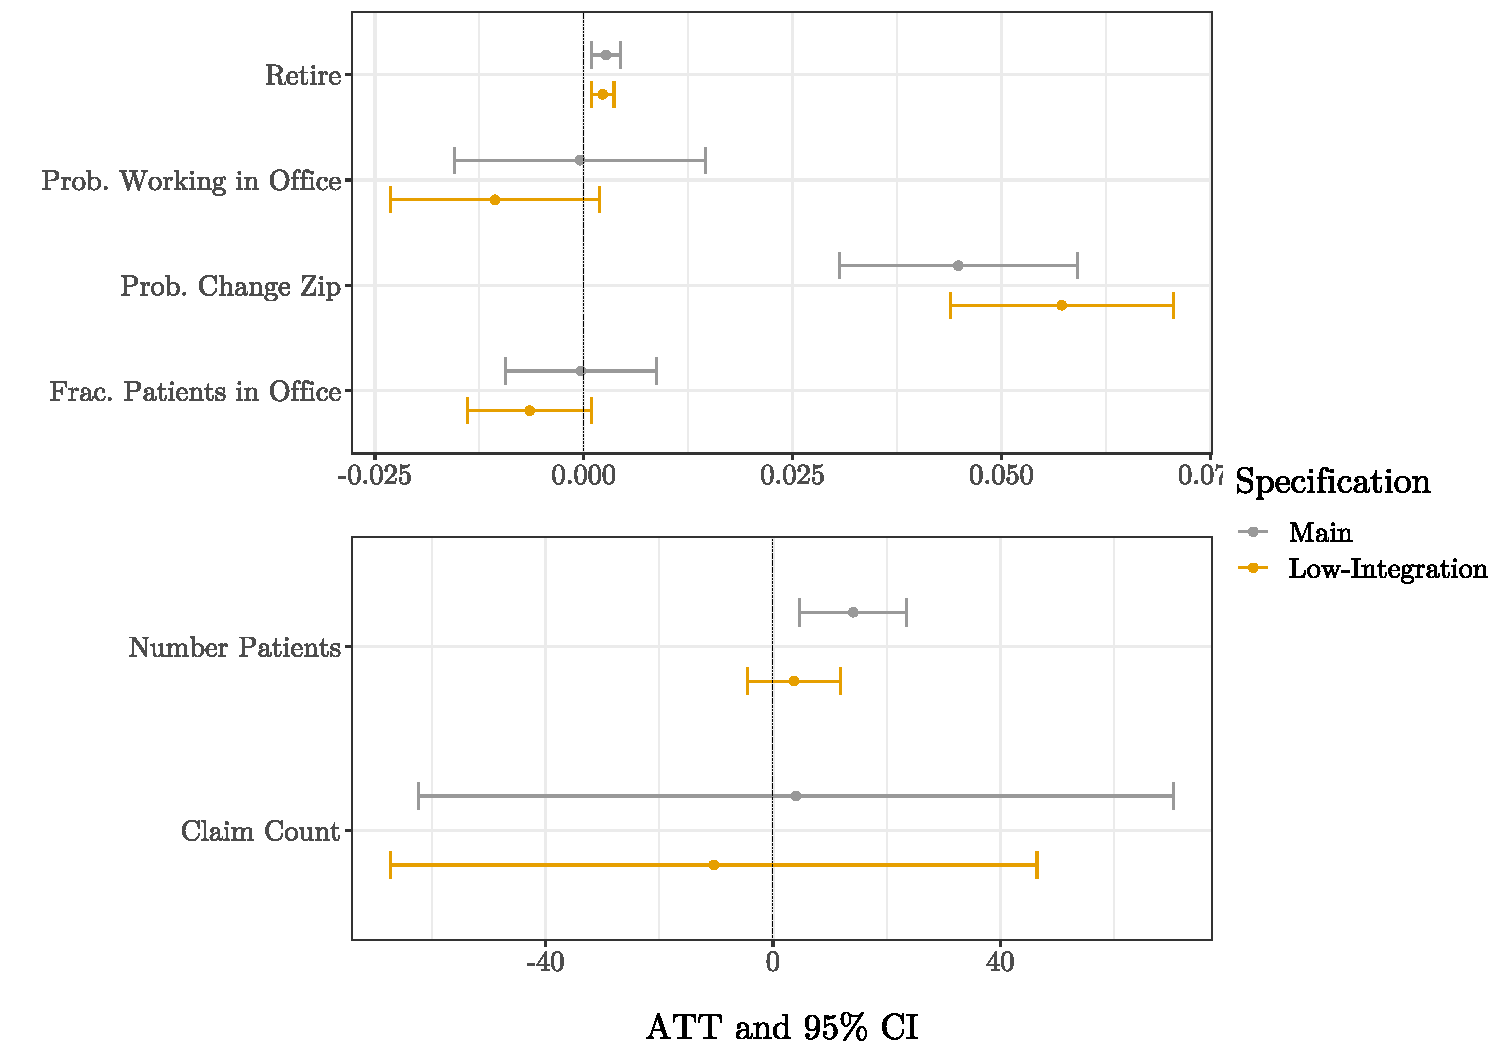
\includegraphics[scale=.57]{Objects/LI_graph.pdf}
    \label{fig:LI}
\end{figure}

\begin{figure}[ht]
    \centering
    \caption{ATT With Anticipation}
    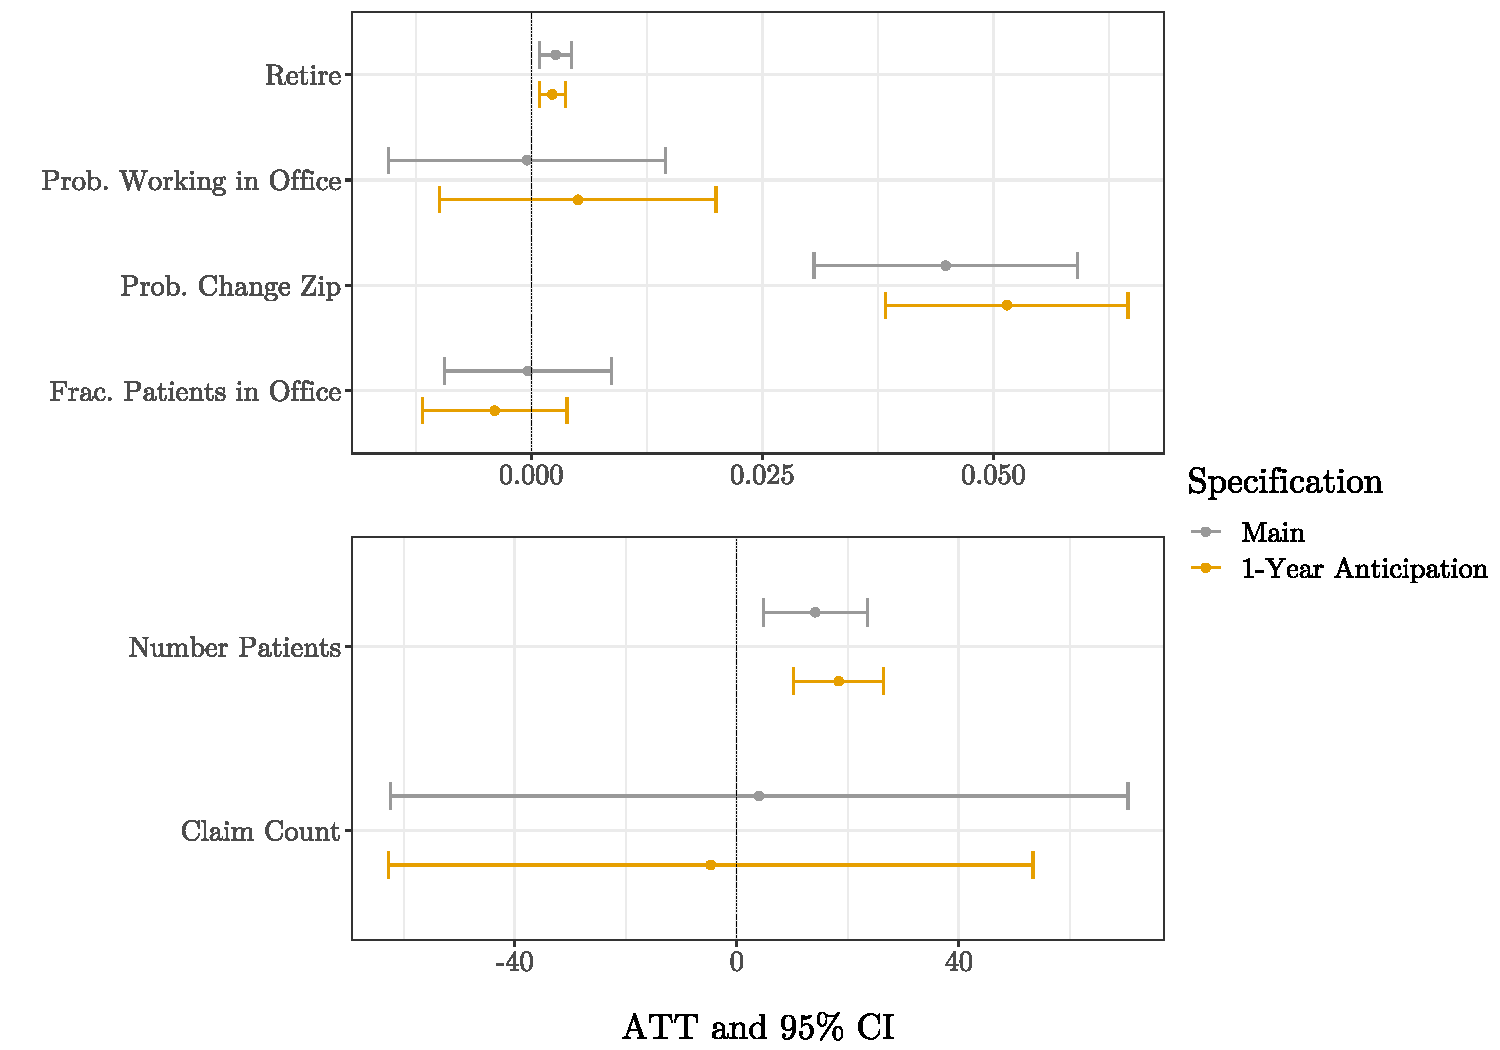
\includegraphics[scale=.57]{Objects/anticipation_graph.pdf}
    \label{fig:anticipation}
\end{figure}

\begin{figure}
    \centering
    \caption{Results: Two Way Fixed Effects}
    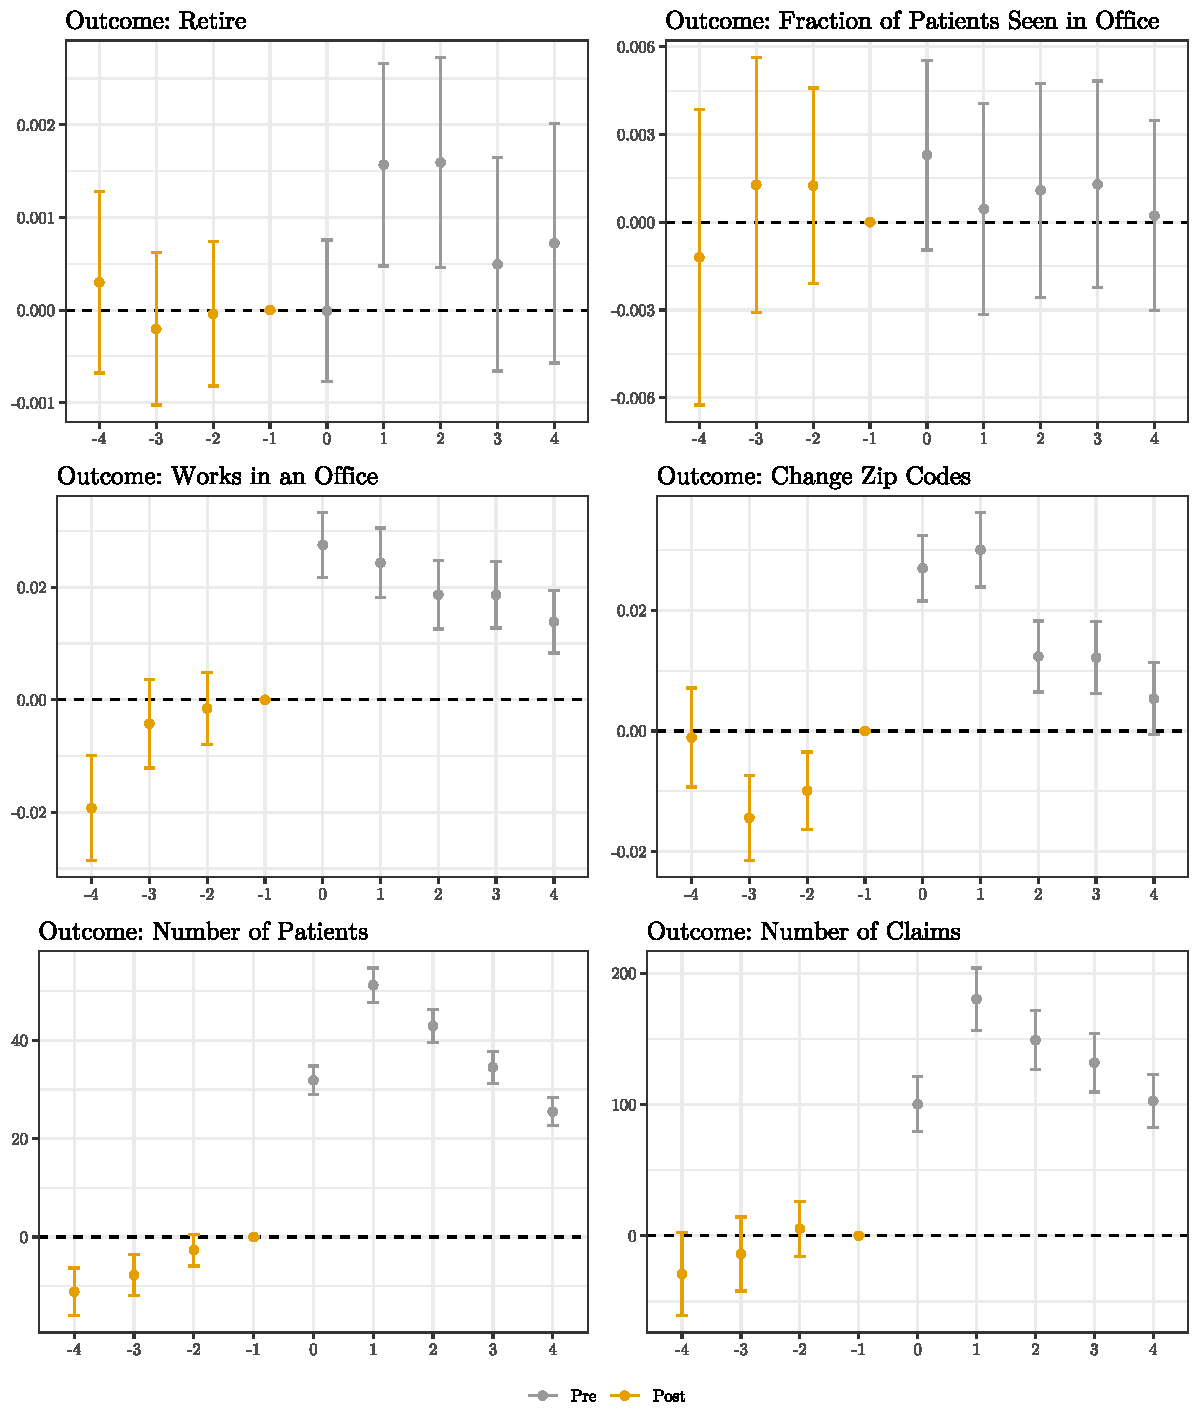
\includegraphics[scale=.8]{Objects/twfe_plot.pdf}
    \label{fig:twfe}
\end{figure}

\begin{figure}[ht]
    \centering
    \caption{Other Event Study Estimators}
    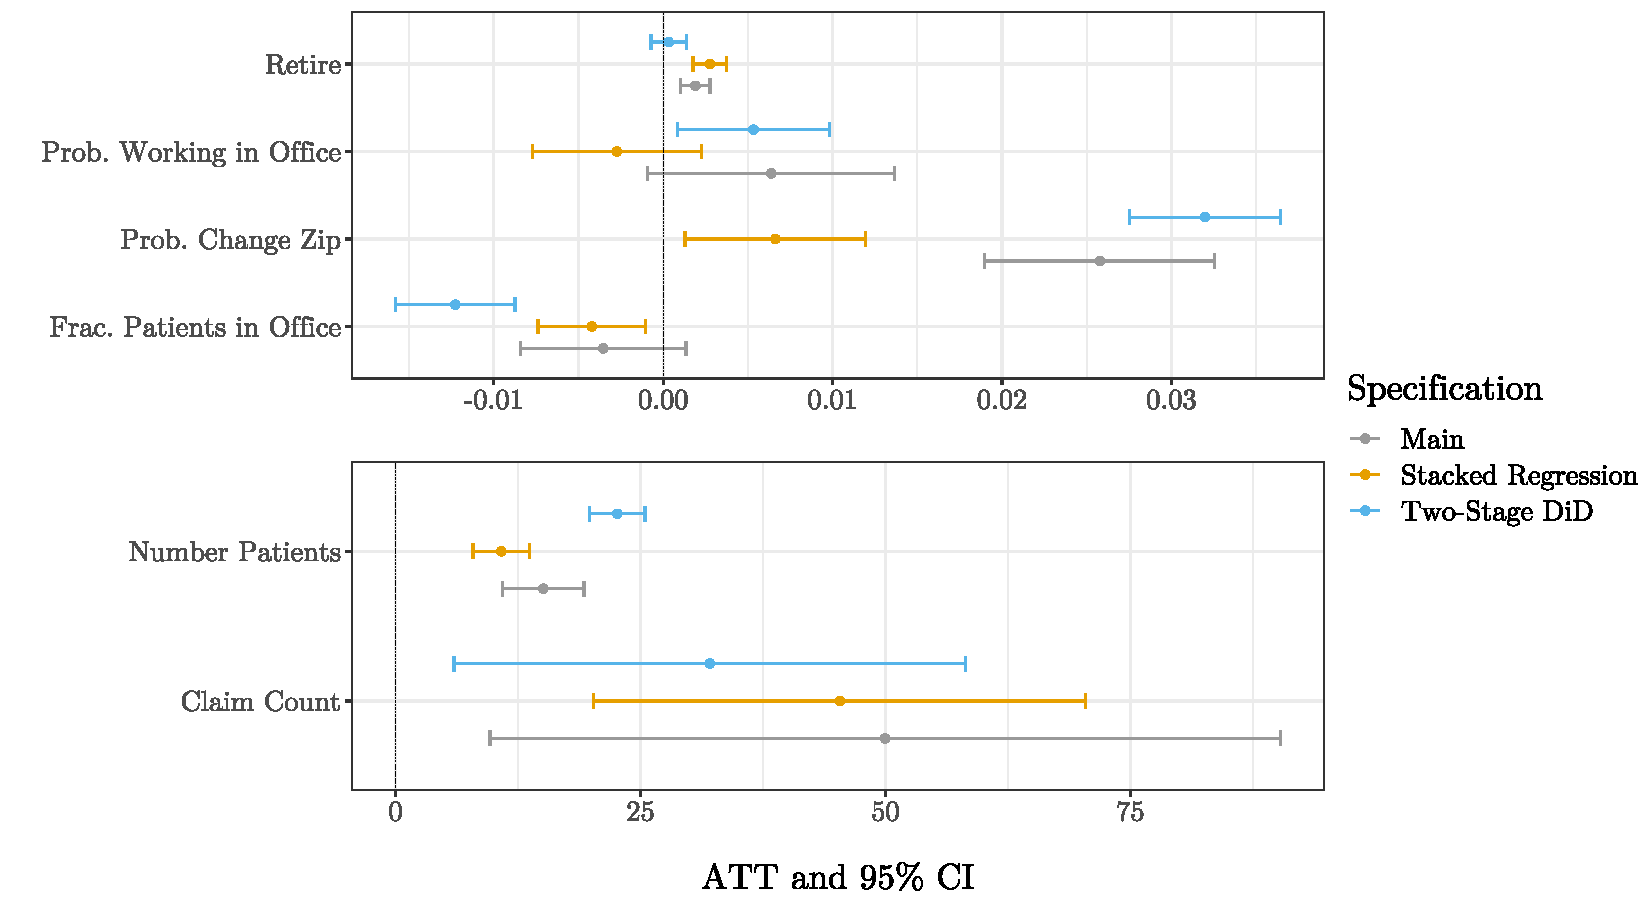
\includegraphics[scale=.57]{Objects/estimators_graph.pdf}
    \label{fig:esimators}
\end{figure}

\begin{figure}[ht]
    \centering
    \caption{Limited Sample Years}
    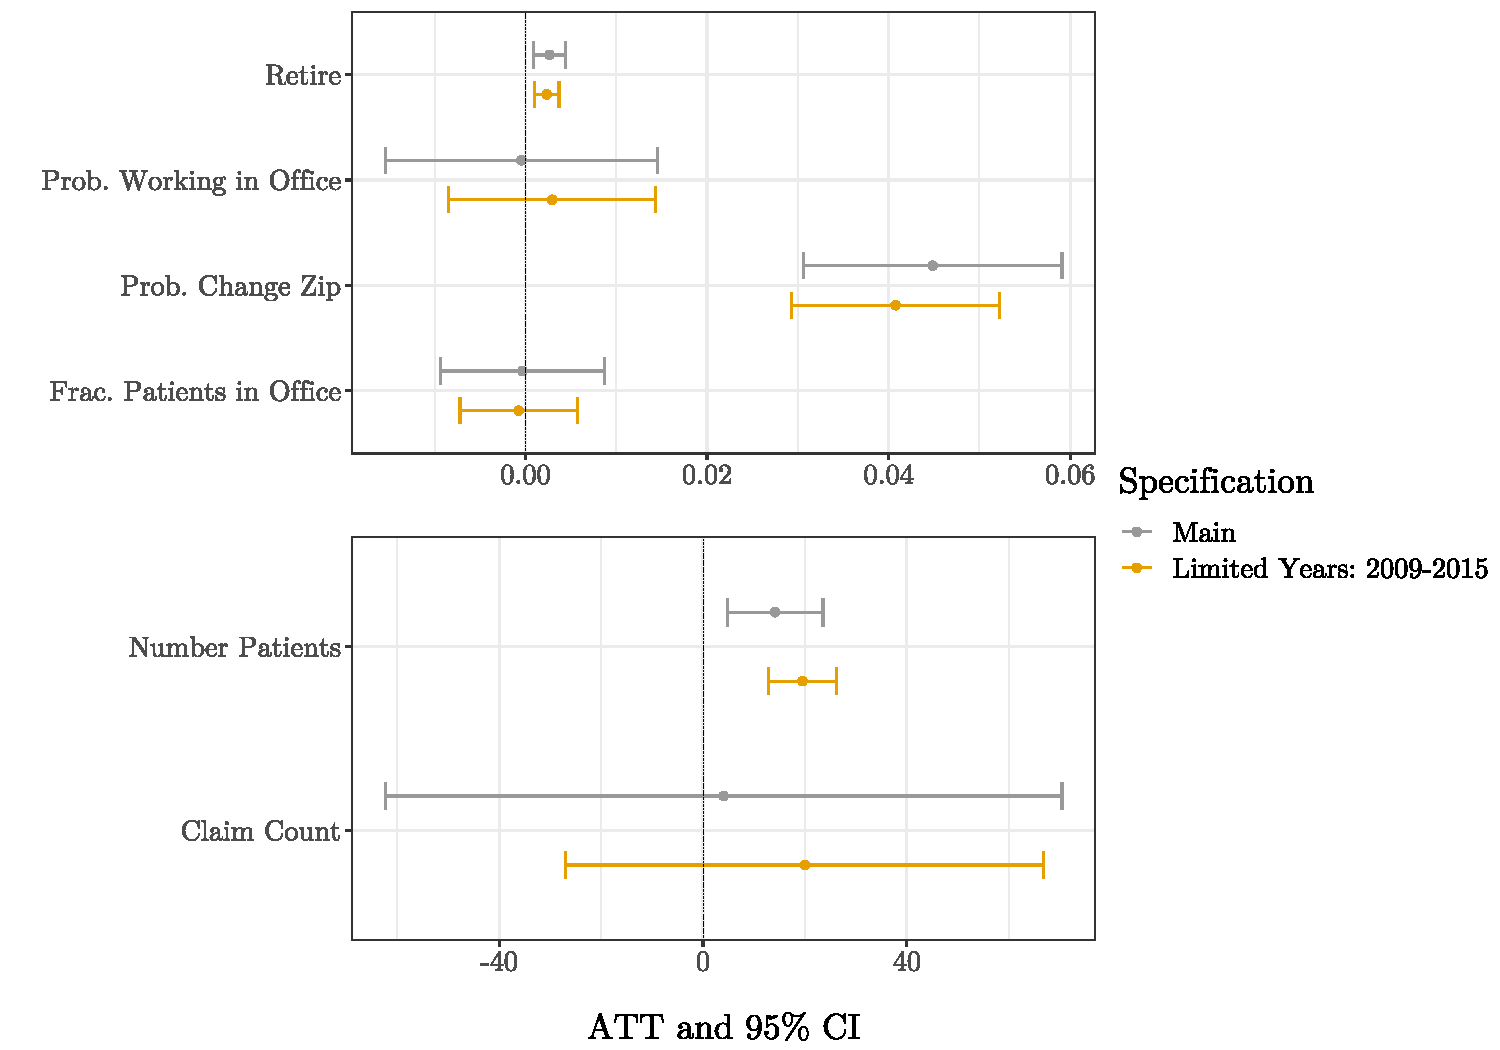
\includegraphics[scale=.5]{Objects/years_graph.pdf}
    \label{fig:years}
\end{figure}

\begin{figure}[ht]
    \centering
    \caption{Physicians without Data Assistants}
    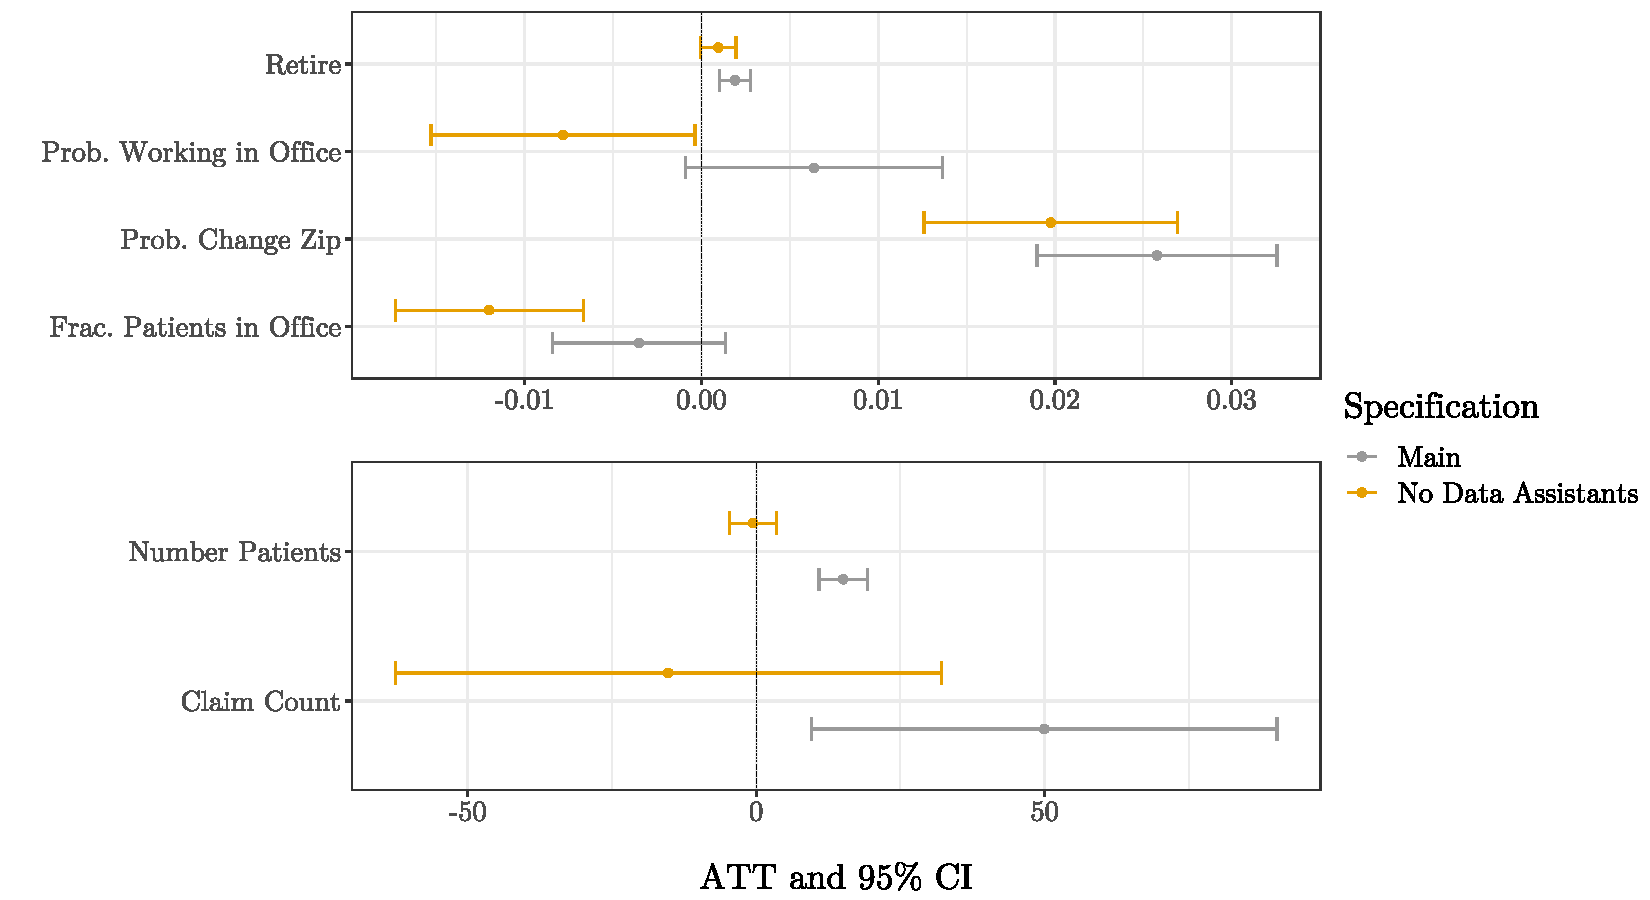
\includegraphics[scale=.57]{Objects/DA_graph.pdf}
    \label{fig:DA}
\end{figure}


\begin{figure}[ht]
    \centering
    \caption{Heterogeneity Analysis}
    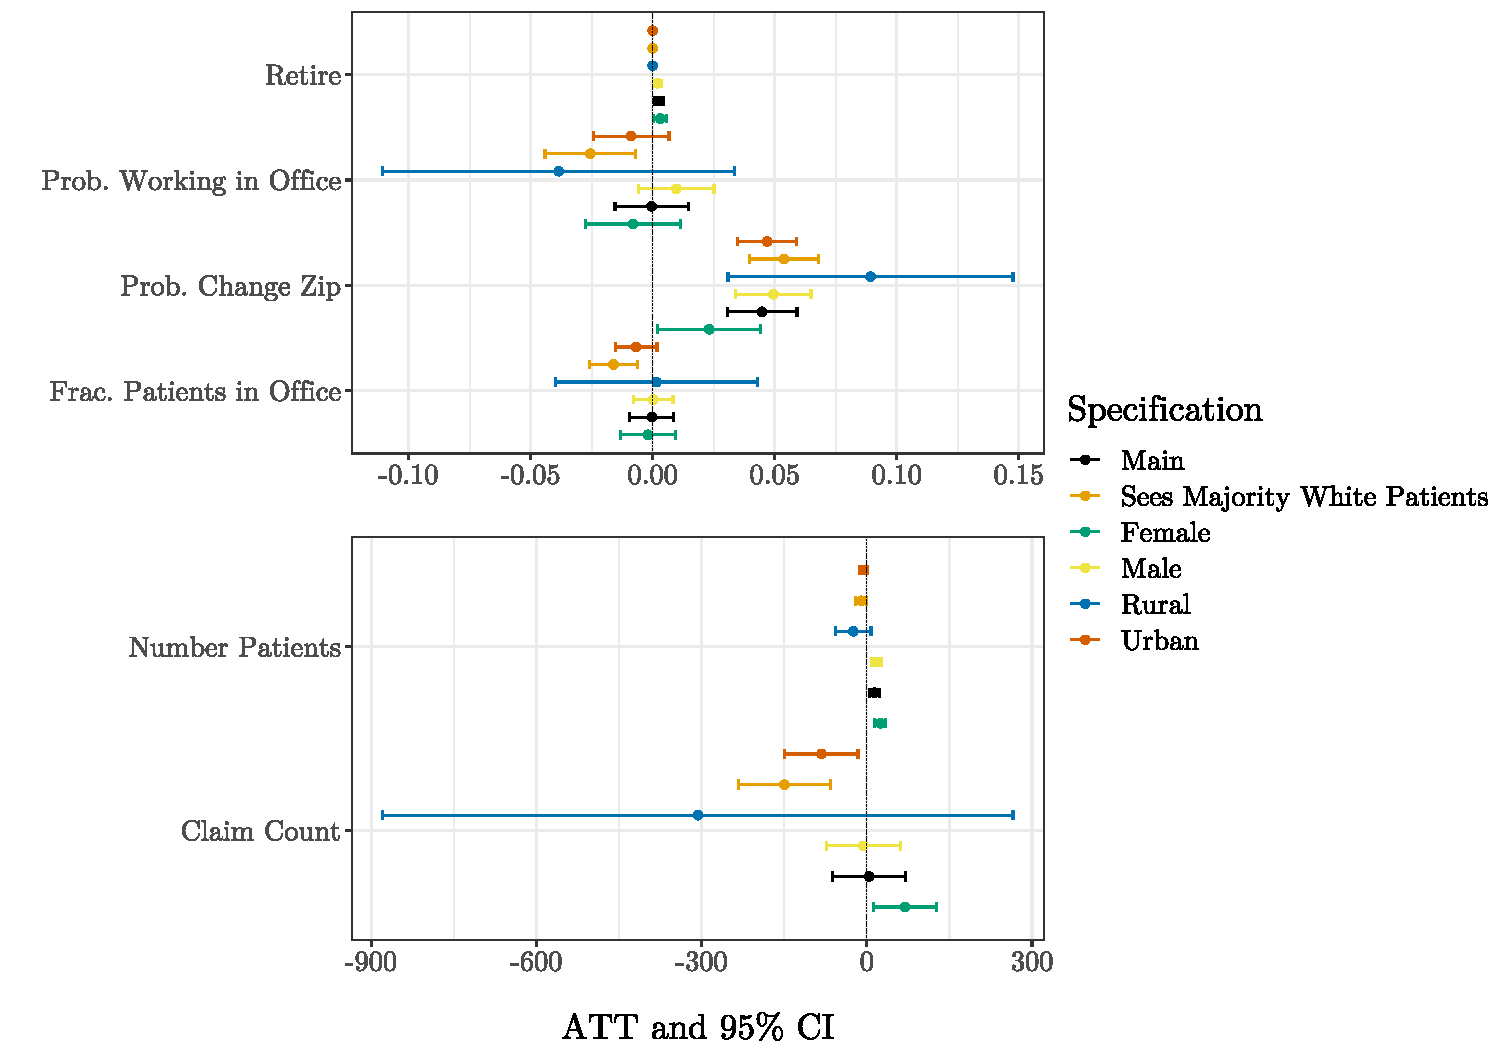
\includegraphics[scale=.57]{Objects/heterogeneity _graph.pdf}
    \label{fig:het}
\end{figure}
















\end{document}